% Options for packages loaded elsewhere
\PassOptionsToPackage{unicode}{hyperref}
\PassOptionsToPackage{hyphens}{url}
%
\documentclass[
]{book}
\usepackage{lmodern}
\usepackage{amssymb,amsmath}
\usepackage{ifxetex,ifluatex}
\ifnum 0\ifxetex 1\fi\ifluatex 1\fi=0 % if pdftex
  \usepackage[T1]{fontenc}
  \usepackage[utf8]{inputenc}
  \usepackage{textcomp} % provide euro and other symbols
\else % if luatex or xetex
  \usepackage{unicode-math}
  \defaultfontfeatures{Scale=MatchLowercase}
  \defaultfontfeatures[\rmfamily]{Ligatures=TeX,Scale=1}
\fi
% Use upquote if available, for straight quotes in verbatim environments
\IfFileExists{upquote.sty}{\usepackage{upquote}}{}
\IfFileExists{microtype.sty}{% use microtype if available
  \usepackage[]{microtype}
  \UseMicrotypeSet[protrusion]{basicmath} % disable protrusion for tt fonts
}{}
\makeatletter
\@ifundefined{KOMAClassName}{% if non-KOMA class
  \IfFileExists{parskip.sty}{%
    \usepackage{parskip}
  }{% else
    \setlength{\parindent}{0pt}
    \setlength{\parskip}{6pt plus 2pt minus 1pt}}
}{% if KOMA class
  \KOMAoptions{parskip=half}}
\makeatother
\usepackage{xcolor}
\IfFileExists{xurl.sty}{\usepackage{xurl}}{} % add URL line breaks if available
\IfFileExists{bookmark.sty}{\usepackage{bookmark}}{\usepackage{hyperref}}
\hypersetup{
  pdftitle={Presentation of Tables, Graphs and Maps},
  pdfauthor={Alex Thomson},
  hidelinks,
  pdfcreator={LaTeX via pandoc}}
\urlstyle{same} % disable monospaced font for URLs
\usepackage{color}
\usepackage{fancyvrb}
\newcommand{\VerbBar}{|}
\newcommand{\VERB}{\Verb[commandchars=\\\{\}]}
\DefineVerbatimEnvironment{Highlighting}{Verbatim}{commandchars=\\\{\}}
% Add ',fontsize=\small' for more characters per line
\usepackage{framed}
\definecolor{shadecolor}{RGB}{248,248,248}
\newenvironment{Shaded}{\begin{snugshade}}{\end{snugshade}}
\newcommand{\AlertTok}[1]{\textcolor[rgb]{0.94,0.16,0.16}{#1}}
\newcommand{\AnnotationTok}[1]{\textcolor[rgb]{0.56,0.35,0.01}{\textbf{\textit{#1}}}}
\newcommand{\AttributeTok}[1]{\textcolor[rgb]{0.77,0.63,0.00}{#1}}
\newcommand{\BaseNTok}[1]{\textcolor[rgb]{0.00,0.00,0.81}{#1}}
\newcommand{\BuiltInTok}[1]{#1}
\newcommand{\CharTok}[1]{\textcolor[rgb]{0.31,0.60,0.02}{#1}}
\newcommand{\CommentTok}[1]{\textcolor[rgb]{0.56,0.35,0.01}{\textit{#1}}}
\newcommand{\CommentVarTok}[1]{\textcolor[rgb]{0.56,0.35,0.01}{\textbf{\textit{#1}}}}
\newcommand{\ConstantTok}[1]{\textcolor[rgb]{0.00,0.00,0.00}{#1}}
\newcommand{\ControlFlowTok}[1]{\textcolor[rgb]{0.13,0.29,0.53}{\textbf{#1}}}
\newcommand{\DataTypeTok}[1]{\textcolor[rgb]{0.13,0.29,0.53}{#1}}
\newcommand{\DecValTok}[1]{\textcolor[rgb]{0.00,0.00,0.81}{#1}}
\newcommand{\DocumentationTok}[1]{\textcolor[rgb]{0.56,0.35,0.01}{\textbf{\textit{#1}}}}
\newcommand{\ErrorTok}[1]{\textcolor[rgb]{0.64,0.00,0.00}{\textbf{#1}}}
\newcommand{\ExtensionTok}[1]{#1}
\newcommand{\FloatTok}[1]{\textcolor[rgb]{0.00,0.00,0.81}{#1}}
\newcommand{\FunctionTok}[1]{\textcolor[rgb]{0.00,0.00,0.00}{#1}}
\newcommand{\ImportTok}[1]{#1}
\newcommand{\InformationTok}[1]{\textcolor[rgb]{0.56,0.35,0.01}{\textbf{\textit{#1}}}}
\newcommand{\KeywordTok}[1]{\textcolor[rgb]{0.13,0.29,0.53}{\textbf{#1}}}
\newcommand{\NormalTok}[1]{#1}
\newcommand{\OperatorTok}[1]{\textcolor[rgb]{0.81,0.36,0.00}{\textbf{#1}}}
\newcommand{\OtherTok}[1]{\textcolor[rgb]{0.56,0.35,0.01}{#1}}
\newcommand{\PreprocessorTok}[1]{\textcolor[rgb]{0.56,0.35,0.01}{\textit{#1}}}
\newcommand{\RegionMarkerTok}[1]{#1}
\newcommand{\SpecialCharTok}[1]{\textcolor[rgb]{0.00,0.00,0.00}{#1}}
\newcommand{\SpecialStringTok}[1]{\textcolor[rgb]{0.31,0.60,0.02}{#1}}
\newcommand{\StringTok}[1]{\textcolor[rgb]{0.31,0.60,0.02}{#1}}
\newcommand{\VariableTok}[1]{\textcolor[rgb]{0.00,0.00,0.00}{#1}}
\newcommand{\VerbatimStringTok}[1]{\textcolor[rgb]{0.31,0.60,0.02}{#1}}
\newcommand{\WarningTok}[1]{\textcolor[rgb]{0.56,0.35,0.01}{\textbf{\textit{#1}}}}
\usepackage{longtable,booktabs}
% Correct order of tables after \paragraph or \subparagraph
\usepackage{etoolbox}
\makeatletter
\patchcmd\longtable{\par}{\if@noskipsec\mbox{}\fi\par}{}{}
\makeatother
% Allow footnotes in longtable head/foot
\IfFileExists{footnotehyper.sty}{\usepackage{footnotehyper}}{\usepackage{footnote}}
\makesavenoteenv{longtable}
\usepackage{graphicx,grffile}
\makeatletter
\def\maxwidth{\ifdim\Gin@nat@width>\linewidth\linewidth\else\Gin@nat@width\fi}
\def\maxheight{\ifdim\Gin@nat@height>\textheight\textheight\else\Gin@nat@height\fi}
\makeatother
% Scale images if necessary, so that they will not overflow the page
% margins by default, and it is still possible to overwrite the defaults
% using explicit options in \includegraphics[width, height, ...]{}
\setkeys{Gin}{width=\maxwidth,height=\maxheight,keepaspectratio}
% Set default figure placement to htbp
\makeatletter
\def\fps@figure{htbp}
\makeatother
\setlength{\emergencystretch}{3em} % prevent overfull lines
\providecommand{\tightlist}{%
  \setlength{\itemsep}{0pt}\setlength{\parskip}{0pt}}
\setcounter{secnumdepth}{5}
\usepackage{booktabs}
\usepackage{amsthm}
\makeatletter
\def\thm@space@setup{%
  \thm@preskip=8pt plus 2pt minus 4pt
  \thm@postskip=\thm@preskip
}
\makeatother
\usepackage{fontspec}
\usepackage{multirow}
\usepackage{multicol}
\usepackage{colortbl}
\usepackage{hhline}
\usepackage{longtable}
\usepackage{array}
\usepackage{hyperref}
\usepackage[]{natbib}
\bibliographystyle{apalike}

\title{Presentation of Tables, Graphs and Maps}
\author{Alex Thomson}
\date{2021-07-14}

\begin{document}
\maketitle

{
\setcounter{tocdepth}{1}
\tableofcontents
}
\hypertarget{introduction}{%
\chapter{Introduction}\label{introduction}}

Visualising data is an essential part of communicating messages and results to any form of audience. An ineffective visualisation of data can communicate a very misleading message.

Building skills in data visualisation can help you to understand and see important results in other people's tables, graphs, and maps. This is in addition to enabling you to create informative visualisations of your own.

The aim of this document is to provide comprehensive guidance on the presentation of data in tables, graphs, and maps. This will include both general guidance and more specific advice on different types of visualisations. We intend to provide some principles of good graphical, tabular, and cartographic practice. By providing this advice, we hope to assist anyone in their future work, especially when it comes to the writing up of research results for an audience.

This guide is intended for anyone who wishes to develop their data visualisation and reporting skills. The advice presented here will be applicable to a wide variety of situations and is not specific to certain topics. Additionally, we hope that users of all ability levels will be able to take this advice to mind in their future projects and their everyday interactions with data.

This resource will start by exploring some general guidance on the presentation of data before going into more specific detail on the use of tables, graphs and maps (an increasingly popular method of presenting data). It then provides advice on ensuring your visualisations are accessible, with consideration on the use of colour.

\hypertarget{gg}{%
\chapter{General Guidance}\label{gg}}

Through developing your data visualisation skills, you can generate a wide variety of graphical/cartographic/tabular representations of data. This could be anything from simple bar graphs and line graphs to complicated cartograms. However, regardless of the complexity of your chosen data visualisation technique, there are certain principles that should always be followed:

\hypertarget{effectiveness}{%
\section{Effectiveness}\label{effectiveness}}

By effectiveness, we mean you should be ensuring that you are using the right type of visualisation for your objectives and priorities. This is the first crucial step in making sure what you produce is effective at displaying the message you intend to show. If you pick the wrong method, your visualisation will not be effective regardless of its quality.

Maps are of course for displaying data which have some form of geographic component.

Tables are suited for presenting structured numerical information; consider tables of means across some groups, frequencies, or some statistical information. This makes them ideal for when the message is in the specific numbers and potentially the relationship between them.

Graphs are quite multi-purpose; there is a type of graph for almost any message you could be wanting to convey. In general, we would choose to use them for indicating trends, making broad comparisons, or showing relationships.

\hypertarget{readability}{%
\section{Readability}\label{readability}}

All elements of your visualisation should be legible, understandable, and coherent. In a word, readable. While this largely relates to any textual elements of your visualisations, the principle is applicable to the whole visualisation.

This includes having titles and headings which concisely explain the content. It should be informative without being overly long and confusing. The same goes for any further labels such as axis labels for graphs, column headings for tables and geographic labels on a map.

Details to consider mentioning include measurement units, geographical coverage, time, the source of the data and any relevant statistics.
Of course, the elements of a visualisation will vary depending on what visual you produce, but they should always be easy to read and understand. You can achieve this by avoiding language beyond the scope of your target audience, providing the necessary information needed to read your visual and presenting the element in a simple and tidy manner. You will find further guidance on specific elements in each of the subsequent sections of this guide.

\hypertarget{tidiness}{%
\section{Tidiness}\label{tidiness}}

A visualisation should never be cluttered. This follows on from readability, although more specifically relates to positioning and spacing of elements as well as avoiding using unnecessary elements.

This includes making sure no elements are overlapping; there should be adequate spacing between them without there being so much that it makes the visualisation look empty. This can also be described as making good use of ``white space''.

There is much more to be said on this topic, but these are mostly specific to the type of visualisation you are using. The general principle of ensuring your visual is neat and organised is always applicable.

\hypertarget{accessibility}{%
\section{Accessibility}\label{accessibility}}

Accessibility has become an increasingly important aspect of data presentation in recent years. Ensuring good practice in accessibility will help in getting an even wider audience to see our research and use our results. The Government Statistical Service makes content accessible to those with impairments to their vision, hearing, mobility, and thinking/understanding skills. For our purposes, we are mostly concerned with visual impairments.

There are some general principles on accessibility, including making sure you explain any uncommon abbreviations, avoiding clutter and keeping information concise. However, we are focusing on the use of colour. Further guidance on this is included in the accessibility section of this document. This includes considerations of colour blindness, cultural context, and the use of saturation/hue/luminance.

\hypertarget{consistency}{%
\section{Consistency}\label{consistency}}

This is mostly relevant when you are intending to use multiple visualisations across your report. When doing so, it is important to ensure you maintain a level of internal consistency.

This involves many aspects. For instance, if you intend to disaggregate your visuals by the levels of a variable, pay attention to the order you put these categories in. They should be kept to a logical or ascending/descending order and this order should be kept the same for the sake of consistency and readability.

The same goes for when using colours to indicate certain characteristics of the data; keep the meaning of the colours consistent.

Of course, this is also important for all the smaller details such as the font, size and face (bold/italic) of text. In essence, try to keep the formatting between visualisations as similar as possible. Generate your personal visual style and stick to it. Changing things up too much will just confuse your audience and reduce your visual's readability.

\hypertarget{informative}{%
\section{Informative}\label{informative}}

A good data visualisation serves to succinctly show a message about our findings. We aim to inform our reader. Usually, it would be accompanied by some text which helps to interpret the visualisation, placing it into a wider context or providing more formal details such as the results of a relevant statistical analysis.

However, a good data visualisation should be self-explanatory and should be able to serve as a stand-alone piece. The reader should be able to understand the message without constantly referring to the text. Much of this can be accomplished by sticking to the particulars of keeping your visual tidy and readable.

Whenever creating a table, graph, or a map, you should include the source of the information from which the visualisation was created. This aids the credibility of your visualisation but also ensures a properly informed audience. An exception is when all information that is used for visualisations in a report comes from the same source. In this case, you should clearly indicate the source in advance of your visualisations.
This also means making sure that your visual is necessary in the first place. Consider the following: Can you achieve the same message with some simple text? Can a visualisation accurately demonstrate your results, or would it be distracting? Are your results too complex to visualise in isolation?

These six principles are relevant regardless of which visualisation you choose to create. In the following sections you will find guidance that is more specific to tables, graphs, and maps. While the guidance is specific to the different forms, they all tie into the central principles described here in this first section.

\hypertarget{CTM}{%
\chapter{Considering the Message}\label{CTM}}

Two of the above principles go beyond the specifics of what you put into your data visualisations: effectiveness and being informative. Consideration of these two principles does not start when you plot your variables. They are principles which should guide your entire research process, including presentation.

This guide will make regular reference to considering what is appropriate for your message, your results and your purpose. For your data visualisations to be effective and informative, you need to think hard about the message you want them to convey. This will often come back to an original research question. These research questions should always be guiding you in the creation of data visualisations. Effective data presentation needs to have something to say, and what it says should be relevant.

Consider this as a process:

\begin{enumerate}
\def\labelenumi{\arabic{enumi}.}
\item
  We start with our research questions that we want to help answer through our research.
\item
  We can break these up and consider how we will answer them. What are going to be the key points we will need to investigate to answer these questions?
\end{enumerate}

For example, say we want to research the prevalence of a disease across areas within a country. We can decide that we are going to need to make points about the overall prevalence, the geographical variation, the explanations, compounding variables. We could look at these as the building blocks of our messages. Our messages are what we want people to remember and they will all stack up to help answer our bigger questions.

\begin{enumerate}
\def\labelenumi{\arabic{enumi}.}
\setcounter{enumi}{2}
\item
  After this, we conduct our analysis and pick out our key findings. These key findings will similarly be informed by our existing research questions and pre-conceived ideas about what our messages will be. However, they should always be flexible; an unexpected result should not be ignored.
\item
  We now need to update our messages based on what we have observed. Our messages should always strive to be important, relevant, and interesting. Also consider novelty; repeating a message we have heard many times over and over will not result in a very interesting data visualisation.
\item
  These updated messages and key findings will inform the creation of our presentable data visualisations. These visualisations along with our messages help to answer our initial research questions.
\end{enumerate}

Therefore, we think about being effective and informative throughout the research process. If your messages and questions are not effective or informative then you cannot expect your visualisations to be.

Bringing effectiveness and informativeness into your data visualisations requires careful consideration of the messages you have drafted. This leads to questions you will need to ask of yourself, including:

\begin{itemize}
\tightlist
\item
  What variables should I include?
\end{itemize}

You should not be including more variables than are necessary. Think about the specifics of your intended message and only include the variables which are relevant and necessary for effectively showing this message. You should also avoid including variables which are uninformative. If adding in a variable does not add any explanatory value, then drop it from your visualisation.

\begin{itemize}
\tightlist
\item
  Which variables should I split by?
\end{itemize}

Disaggregating your findings by certain groups is a common practice. What variables you use to do this splitting should largely be informed by your research questions and messages.

Consider the example of geographical variation of disease prevalence. Explicitly, we know we will need to look at how our results vary by geography, but we may also want to consider variables which could help to explain the geographical variation. So, we could split by levels of economic deprivation or rurality. It always comes back to keeping relevant and important.

\begin{itemize}
\tightlist
\item
  Which graph/table/map should I use?
\end{itemize}

This involves thinking carefully about the type of message you want to show.
Does your message mostly concern changes over time? If so, then a table probably is not suitable unless it is quite a short time frame with few points.

A few graphical options would be suitable including line graphs, column charts, slope charts etc. From here, the choice would now be dependent on the types of variables you want to show. Concerned with totals? Then consider column charts. Concerned with averages/rates? Consider a line chart.

Deciding on the right type of graph is a process, starting from your overall message and working down:

\begin{enumerate}
\def\labelenumi{\arabic{enumi}.}
\item
  What is the purpose of your message? (Change over time? Distribution? Spatial? Correlation? Etc.)
\item
  What variables are you plotting and how many? (Categorical? Continuous?)
\item
  How much data needs displaying? A lot or a little?
\item
  What are the measurement units? (Averages? Totals? Rates? Proportions?)
\end{enumerate}

Considering these questions should help you to narrow down what type of data visualisation is most appropriate. There are too many possible variations to consider here, but these points should help guide your thinking process.

\hypertarget{tables}{%
\chapter{Tables}\label{tables}}

When thinking of data visualisations, tables may not be your first choice as they are not as visually remarkable as a graph. However, tables are a crucial tool in presenting data and results as they have the advantage of much greater specificity than graphs and are usually simple to understand. Generally, it is harder to read patterns in tables than in graphs. Therefore, graphs should be used when you want to focus on patterns, trends and relationships that do not necessarily require the exact values to be understood.

A table would therefore be more appropriate than a graph or map if:

\begin{itemize}
\item
  You are asking the audience to compare individual values directly
\item
  You are wanting to include both the values and some derived measures such as percentages or indices. These are harder to show succinctly all together on one graph.
\item
  You want to include summary statistics such as means or totals
\item
  You need to show values with very different magnitudes together.
\item
  If users may want to use the data for their own analysis or reference.
\end{itemize}

\textbf{Reference tables} contain extensive information for people to look up.

\begin{itemize}
\tightlist
\item
  They are useful for archival purposes rather than analysis.
\item
  They should include detailed metadata about the information presented: what, where and when of the data.
\item
  They usually appear as appendices.
\end{itemize}

\textbf{Demonstration tables} are probably what you think of when we mention tables for research purposes.

\begin{itemize}
\item
  They are intended to reinforce a point by showing statistics or values that can be quickly assimilated by the reader.
\item
  They are included within the text to allow readers to follow the general argument and without having to flip back and forth to refer to the relevant information.
\item
  It is important they are clear and well-presented, usually using reasonable approximations to keep figures to a few significant figures.
\item
  Very large demonstration tables can be confusing and intimidating. If all the information is truly required, it should be split across multiple smaller tables.
\end{itemize}

The following guidance mostly concerns the formatting of demonstration tables although the general principles are applicable to both forms.

Reference tables however are not designed to draw attention to specific numbers, patterns, or comparisons and therefore advice on topics such as ordering of columns and rows are not especially relevant.

\hypertarget{introduction-to-flextable}{%
\section{Introduction to Flextable}\label{introduction-to-flextable}}

This section of the guide will be supplemented by reproducible code examples from R. These will be focusing on the incredibly useful package flextable which has been designed to help create report ready tables directly in R. It is especially useful for those intending to write their reports or knit their documents into Word format. This guide will mostly cover some of the basic features, for extended guidance on the full capabilities of flextable, please see this \href{https://ardata-fr.github.io/flextable-book/}{guide}

In general, when using flextable the idea is to use R code to manipulate your data into roughly the format you wish to present as a table. In other words you create your table as a data frame. For purposes of demonstration, all data manipulation shown shall be done using the tidyverse range of packages, particularly dplyr and tidyr.

Once you have your data in a desired format you can apply flextable functions to the data to create and design your table. Starting with \texttt{flextable()} to turn your data from a data.frame/tibble object into a flextable object.

A flextable object consists of 3 parts.

\begin{itemize}
\tightlist
\item
  header: the section containing any and all headers/titles (defaults to column names of data frames in a single row)
\item
  body: this contains all of the data from the data frame
\item
  footer: not present by default but can be used to add footnotes or additional content
\end{itemize}

Additionally, in flextable notation \texttt{i} donates rows and \texttt{j} donates columns. Both can be referred to in functions by their row or column number. Note however that the numbering works within parts e.g.~by default the row of column headers is i=1 within the part ``header'', while the first row of data is i=1 within the part ``body''.



\begin{figure}

{\centering 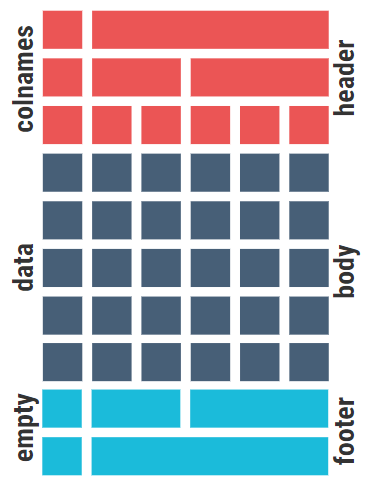
\includegraphics[width=5.18in]{img/flextable_object} 

}

\caption{\href{https://ardata-fr.github.io/flextable-book/design.html\#table-parts}{Structure of a flextable object}}\label{fig:unnamed-chunk-2}
\end{figure}

Flextable can be installed to R in the usual manner from CRAN.

\begin{Shaded}
\begin{Highlighting}[]
\CommentTok{#install.packages("flextable")}

\KeywordTok{library}\NormalTok{(flextable)}
\end{Highlighting}
\end{Shaded}

\hypertarget{general-guidance}{%
\section{General Guidance}\label{general-guidance}}

\hypertarget{title-column-headers-and-labels}{%
\subsection{Title, column headers and labels}\label{title-column-headers-and-labels}}

Titles and labels are very important to the design of a table as they help users understand what is being presented. The titles and labels make sure the table works on its own and can be read within a different context than its original presentation.

You should consider including the following information in tables within either titles, labels, headings or possible footnotes, the choice of which points depends on your data and how important the details are to understanding the information:

\begin{itemize}
\tightlist
\item
  Analysis units (people, households etc.)
\item
  Types of statistics (totals, means etc.)
\item
  Units (thousands, kg, \$)
\item
  Geographical coverage
\item
  Time period
\item
  Source of data
\item
  Key quality information
\end{itemize}

\hypertarget{using-flextable---column-headers-and-titles}{%
\subsubsection{Using Flextable - Column headers and titles}\label{using-flextable---column-headers-and-titles}}

Let's look at how we can start using the flextable package to create report ready tables. Starting with how we can set and edit the titles and column headers of our tables.

First we are going to read in our data.

The first dataset data we are using in this guide is an extract of a survey conducted in Uganda from farmers identified as growing beans.

The dataset contains an extract of 50 responses to 23 of the survey questions, and has been imported to R as a data frame called \texttt{BeanSurvey}.

A summary of the columns in the dataset is below.

\begin{Shaded}
\begin{Highlighting}[]
\NormalTok{BeanSurvey <-}\StringTok{ }\KeywordTok{readRDS}\NormalTok{(}\DataTypeTok{file =} \StringTok{"data/bean_survey.RDS"}\NormalTok{)}
\end{Highlighting}
\end{Shaded}

\providecommand{\docline}[3]{\noalign{\global\setlength{\arrayrulewidth}{#1}}\arrayrulecolor[HTML]{#2}\cline{#3}}

\setlength{\tabcolsep}{8pt}

\renewcommand*{\arraystretch}{1.5}

\begin{table}

\centering

\begin{longtable}{|p{1.96in}|p{3.50in}}



\hhline{>{\arrayrulecolor[HTML]{000000}\global\arrayrulewidth=2pt}->{\arrayrulecolor[HTML]{000000}\global\arrayrulewidth=2pt}-}

\multicolumn{1}{!{\color[HTML]{000000}\vrule width 0pt}>{\raggedright}p{\dimexpr 1.96in+0\tabcolsep+0\arrayrulewidth}}{\fontsize{11}{13}\selectfont{\textcolor[HTML]{000000}{\global\setmainfont{Arial}Column}}} & \multicolumn{1}{!{\color[HTML]{000000}\vrule width 0pt}>{\raggedright}p{\dimexpr 3.5in+0\tabcolsep+0\arrayrulewidth}!{\color[HTML]{000000}\vrule width 0pt}}{\fontsize{11}{13}\selectfont{\textcolor[HTML]{000000}{\global\setmainfont{Arial}Description}}} \\

\noalign{\global\setlength{\arrayrulewidth}{2pt}}\arrayrulecolor[HTML]{000000}\cline{1-2}

\endfirsthead

\hhline{>{\arrayrulecolor[HTML]{000000}\global\arrayrulewidth=2pt}->{\arrayrulecolor[HTML]{000000}\global\arrayrulewidth=2pt}-}

\multicolumn{1}{!{\color[HTML]{000000}\vrule width 0pt}>{\raggedright}p{\dimexpr 1.96in+0\tabcolsep+0\arrayrulewidth}}{\fontsize{11}{13}\selectfont{\textcolor[HTML]{000000}{\global\setmainfont{Arial}Column}}} & \multicolumn{1}{!{\color[HTML]{000000}\vrule width 0pt}>{\raggedright}p{\dimexpr 3.5in+0\tabcolsep+0\arrayrulewidth}!{\color[HTML]{000000}\vrule width 0pt}}{\fontsize{11}{13}\selectfont{\textcolor[HTML]{000000}{\global\setmainfont{Arial}Description}}} \\

\noalign{\global\setlength{\arrayrulewidth}{2pt}}\arrayrulecolor[HTML]{000000}\cline{1-2}\endhead



\multicolumn{1}{!{\color[HTML]{000000}\vrule width 0pt}>{\raggedright}p{\dimexpr 1.96in+0\tabcolsep+0\arrayrulewidth}}{\fontsize{11}{13}\selectfont{\textcolor[HTML]{000000}{\global\setmainfont{Arial}ID}}} & \multicolumn{1}{!{\color[HTML]{000000}\vrule width 0pt}>{\raggedright}p{\dimexpr 3.5in+0\tabcolsep+0\arrayrulewidth}!{\color[HTML]{000000}\vrule width 0pt}}{\fontsize{11}{13}\selectfont{\textcolor[HTML]{000000}{\global\setmainfont{Arial}Farmer ID}}} \\





\multicolumn{1}{!{\color[HTML]{000000}\vrule width 0pt}>{\raggedright}p{\dimexpr 1.96in+0\tabcolsep+0\arrayrulewidth}}{\fontsize{11}{13}\selectfont{\textcolor[HTML]{000000}{\global\setmainfont{Arial}VILLAGE}}} & \multicolumn{1}{!{\color[HTML]{000000}\vrule width 0pt}>{\raggedright}p{\dimexpr 3.5in+0\tabcolsep+0\arrayrulewidth}!{\color[HTML]{000000}\vrule width 0pt}}{\fontsize{11}{13}\selectfont{\textcolor[HTML]{000000}{\global\setmainfont{Arial}Village name}}} \\





\multicolumn{1}{!{\color[HTML]{000000}\vrule width 0pt}>{\raggedright}p{\dimexpr 1.96in+0\tabcolsep+0\arrayrulewidth}}{\fontsize{11}{13}\selectfont{\textcolor[HTML]{000000}{\global\setmainfont{Arial}HHTYPE}}} & \multicolumn{1}{!{\color[HTML]{000000}\vrule width 0pt}>{\raggedright}p{\dimexpr 3.5in+0\tabcolsep+0\arrayrulewidth}!{\color[HTML]{000000}\vrule width 0pt}}{\fontsize{11}{13}\selectfont{\textcolor[HTML]{000000}{\global\setmainfont{Arial}Household composition}}} \\





\multicolumn{1}{!{\color[HTML]{000000}\vrule width 0pt}>{\raggedright}p{\dimexpr 1.96in+0\tabcolsep+0\arrayrulewidth}}{\fontsize{11}{13}\selectfont{\textcolor[HTML]{000000}{\global\setmainfont{Arial}GENDERHH}}} & \multicolumn{1}{!{\color[HTML]{000000}\vrule width 0pt}>{\raggedright}p{\dimexpr 3.5in+0\tabcolsep+0\arrayrulewidth}!{\color[HTML]{000000}\vrule width 0pt}}{\fontsize{11}{13}\selectfont{\textcolor[HTML]{000000}{\global\setmainfont{Arial}Gender of Household Head}}} \\





\multicolumn{1}{!{\color[HTML]{000000}\vrule width 0pt}>{\raggedright}p{\dimexpr 1.96in+0\tabcolsep+0\arrayrulewidth}}{\fontsize{11}{13}\selectfont{\textcolor[HTML]{000000}{\global\setmainfont{Arial}AGEHH}}} & \multicolumn{1}{!{\color[HTML]{000000}\vrule width 0pt}>{\raggedright}p{\dimexpr 3.5in+0\tabcolsep+0\arrayrulewidth}!{\color[HTML]{000000}\vrule width 0pt}}{\fontsize{11}{13}\selectfont{\textcolor[HTML]{000000}{\global\setmainfont{Arial}Age of Household Head}}} \\





\multicolumn{1}{!{\color[HTML]{000000}\vrule width 0pt}>{\raggedright}p{\dimexpr 1.96in+0\tabcolsep+0\arrayrulewidth}}{\fontsize{11}{13}\selectfont{\textcolor[HTML]{000000}{\global\setmainfont{Arial}OCCUHH}}} & \multicolumn{1}{!{\color[HTML]{000000}\vrule width 0pt}>{\raggedright}p{\dimexpr 3.5in+0\tabcolsep+0\arrayrulewidth}!{\color[HTML]{000000}\vrule width 0pt}}{\fontsize{11}{13}\selectfont{\textcolor[HTML]{000000}{\global\setmainfont{Arial}Occupation of Household Head}}} \\





\multicolumn{1}{!{\color[HTML]{000000}\vrule width 0pt}>{\raggedright}p{\dimexpr 1.96in+0\tabcolsep+0\arrayrulewidth}}{\fontsize{11}{13}\selectfont{\textcolor[HTML]{000000}{\global\setmainfont{Arial}ADULTS}}} & \multicolumn{1}{!{\color[HTML]{000000}\vrule width 0pt}>{\raggedright}p{\dimexpr 3.5in+0\tabcolsep+0\arrayrulewidth}!{\color[HTML]{000000}\vrule width 0pt}}{\fontsize{11}{13}\selectfont{\textcolor[HTML]{000000}{\global\setmainfont{Arial}Number of Adults within the household}}} \\





\multicolumn{1}{!{\color[HTML]{000000}\vrule width 0pt}>{\raggedright}p{\dimexpr 1.96in+0\tabcolsep+0\arrayrulewidth}}{\fontsize{11}{13}\selectfont{\textcolor[HTML]{000000}{\global\setmainfont{Arial}CHILDREN}}} & \multicolumn{1}{!{\color[HTML]{000000}\vrule width 0pt}>{\raggedright}p{\dimexpr 3.5in+0\tabcolsep+0\arrayrulewidth}!{\color[HTML]{000000}\vrule width 0pt}}{\fontsize{11}{13}\selectfont{\textcolor[HTML]{000000}{\global\setmainfont{Arial}Number of Children (<18) within the household}}} \\





\multicolumn{1}{!{\color[HTML]{000000}\vrule width 0pt}>{\raggedright}p{\dimexpr 1.96in+0\tabcolsep+0\arrayrulewidth}}{\fontsize{11}{13}\selectfont{\textcolor[HTML]{000000}{\global\setmainfont{Arial}MATOKE}}} & \multicolumn{1}{!{\color[HTML]{000000}\vrule width 0pt}>{\raggedright}p{\dimexpr 3.5in+0\tabcolsep+0\arrayrulewidth}!{\color[HTML]{000000}\vrule width 0pt}}{\fontsize{11}{13}\selectfont{\textcolor[HTML]{000000}{\global\setmainfont{Arial}Do they grow matoke?}}} \\





\multicolumn{1}{!{\color[HTML]{000000}\vrule width 0pt}>{\raggedright}p{\dimexpr 1.96in+0\tabcolsep+0\arrayrulewidth}}{\fontsize{11}{13}\selectfont{\textcolor[HTML]{000000}{\global\setmainfont{Arial}MAIZE}}} & \multicolumn{1}{!{\color[HTML]{000000}\vrule width 0pt}>{\raggedright}p{\dimexpr 3.5in+0\tabcolsep+0\arrayrulewidth}!{\color[HTML]{000000}\vrule width 0pt}}{\fontsize{11}{13}\selectfont{\textcolor[HTML]{000000}{\global\setmainfont{Arial}Do they grow maize?}}} \\





\multicolumn{1}{!{\color[HTML]{000000}\vrule width 0pt}>{\raggedright}p{\dimexpr 1.96in+0\tabcolsep+0\arrayrulewidth}}{\fontsize{11}{13}\selectfont{\textcolor[HTML]{000000}{\global\setmainfont{Arial}BEANS}}} & \multicolumn{1}{!{\color[HTML]{000000}\vrule width 0pt}>{\raggedright}p{\dimexpr 3.5in+0\tabcolsep+0\arrayrulewidth}!{\color[HTML]{000000}\vrule width 0pt}}{\fontsize{11}{13}\selectfont{\textcolor[HTML]{000000}{\global\setmainfont{Arial}Do they grow beans?}}} \\





\multicolumn{1}{!{\color[HTML]{000000}\vrule width 0pt}>{\raggedright}p{\dimexpr 1.96in+0\tabcolsep+0\arrayrulewidth}}{\fontsize{11}{13}\selectfont{\textcolor[HTML]{000000}{\global\setmainfont{Arial}BANANA}}} & \multicolumn{1}{!{\color[HTML]{000000}\vrule width 0pt}>{\raggedright}p{\dimexpr 3.5in+0\tabcolsep+0\arrayrulewidth}!{\color[HTML]{000000}\vrule width 0pt}}{\fontsize{11}{13}\selectfont{\textcolor[HTML]{000000}{\global\setmainfont{Arial}Do they grow banana?}}} \\





\multicolumn{1}{!{\color[HTML]{000000}\vrule width 0pt}>{\raggedright}p{\dimexpr 1.96in+0\tabcolsep+0\arrayrulewidth}}{\fontsize{11}{13}\selectfont{\textcolor[HTML]{000000}{\global\setmainfont{Arial}CASSAVA}}} & \multicolumn{1}{!{\color[HTML]{000000}\vrule width 0pt}>{\raggedright}p{\dimexpr 3.5in+0\tabcolsep+0\arrayrulewidth}!{\color[HTML]{000000}\vrule width 0pt}}{\fontsize{11}{13}\selectfont{\textcolor[HTML]{000000}{\global\setmainfont{Arial}Do they grow cassava?}}} \\





\multicolumn{1}{!{\color[HTML]{000000}\vrule width 0pt}>{\raggedright}p{\dimexpr 1.96in+0\tabcolsep+0\arrayrulewidth}}{\fontsize{11}{13}\selectfont{\textcolor[HTML]{000000}{\global\setmainfont{Arial}COFFEE}}} & \multicolumn{1}{!{\color[HTML]{000000}\vrule width 0pt}>{\raggedright}p{\dimexpr 3.5in+0\tabcolsep+0\arrayrulewidth}!{\color[HTML]{000000}\vrule width 0pt}}{\fontsize{11}{13}\selectfont{\textcolor[HTML]{000000}{\global\setmainfont{Arial}Do they grow coffee?}}} \\





\multicolumn{1}{!{\color[HTML]{000000}\vrule width 0pt}>{\raggedright}p{\dimexpr 1.96in+0\tabcolsep+0\arrayrulewidth}}{\fontsize{11}{13}\selectfont{\textcolor[HTML]{000000}{\global\setmainfont{Arial}LANDAREA}}} & \multicolumn{1}{!{\color[HTML]{000000}\vrule width 0pt}>{\raggedright}p{\dimexpr 3.5in+0\tabcolsep+0\arrayrulewidth}!{\color[HTML]{000000}\vrule width 0pt}}{\fontsize{11}{13}\selectfont{\textcolor[HTML]{000000}{\global\setmainfont{Arial}Land area of farm (acres)}}} \\





\multicolumn{1}{!{\color[HTML]{000000}\vrule width 0pt}>{\raggedright}p{\dimexpr 1.96in+0\tabcolsep+0\arrayrulewidth}}{\fontsize{11}{13}\selectfont{\textcolor[HTML]{000000}{\global\setmainfont{Arial}LABOR}}} & \multicolumn{1}{!{\color[HTML]{000000}\vrule width 0pt}>{\raggedright}p{\dimexpr 3.5in+0\tabcolsep+0\arrayrulewidth}!{\color[HTML]{000000}\vrule width 0pt}}{\fontsize{11}{13}\selectfont{\textcolor[HTML]{000000}{\global\setmainfont{Arial}Labor usage}}} \\





\multicolumn{1}{!{\color[HTML]{000000}\vrule width 0pt}>{\raggedright}p{\dimexpr 1.96in+0\tabcolsep+0\arrayrulewidth}}{\fontsize{11}{13}\selectfont{\textcolor[HTML]{000000}{\global\setmainfont{Arial}INTERCROP}}} & \multicolumn{1}{!{\color[HTML]{000000}\vrule width 0pt}>{\raggedright}p{\dimexpr 3.5in+0\tabcolsep+0\arrayrulewidth}!{\color[HTML]{000000}\vrule width 0pt}}{\fontsize{11}{13}\selectfont{\textcolor[HTML]{000000}{\global\setmainfont{Arial}Intercrops with beans}}} \\





\multicolumn{1}{!{\color[HTML]{000000}\vrule width 0pt}>{\raggedright}p{\dimexpr 1.96in+0\tabcolsep+0\arrayrulewidth}}{\fontsize{11}{13}\selectfont{\textcolor[HTML]{000000}{\global\setmainfont{Arial}DECISIONS}}} & \multicolumn{1}{!{\color[HTML]{000000}\vrule width 0pt}>{\raggedright}p{\dimexpr 3.5in+0\tabcolsep+0\arrayrulewidth}!{\color[HTML]{000000}\vrule width 0pt}}{\fontsize{11}{13}\selectfont{\textcolor[HTML]{000000}{\global\setmainfont{Arial}Household decision responsibility}}} \\





\multicolumn{1}{!{\color[HTML]{000000}\vrule width 0pt}>{\raggedright}p{\dimexpr 1.96in+0\tabcolsep+0\arrayrulewidth}}{\fontsize{11}{13}\selectfont{\textcolor[HTML]{000000}{\global\setmainfont{Arial}SELLBEANS}}} & \multicolumn{1}{!{\color[HTML]{000000}\vrule width 0pt}>{\raggedright}p{\dimexpr 3.5in+0\tabcolsep+0\arrayrulewidth}!{\color[HTML]{000000}\vrule width 0pt}}{\fontsize{11}{13}\selectfont{\textcolor[HTML]{000000}{\global\setmainfont{Arial}Do they grow beans for sale?}}} \\





\multicolumn{1}{!{\color[HTML]{000000}\vrule width 0pt}>{\raggedright}p{\dimexpr 1.96in+0\tabcolsep+0\arrayrulewidth}}{\fontsize{11}{13}\selectfont{\textcolor[HTML]{000000}{\global\setmainfont{Arial}BEANSPLANTED\_LR}}} & \multicolumn{1}{!{\color[HTML]{000000}\vrule width 0pt}>{\raggedright}p{\dimexpr 3.5in+0\tabcolsep+0\arrayrulewidth}!{\color[HTML]{000000}\vrule width 0pt}}{\fontsize{11}{13}\selectfont{\textcolor[HTML]{000000}{\global\setmainfont{Arial}Quantity of beans planted in long rain season}}} \\





\multicolumn{1}{!{\color[HTML]{000000}\vrule width 0pt}>{\raggedright}p{\dimexpr 1.96in+0\tabcolsep+0\arrayrulewidth}}{\fontsize{11}{13}\selectfont{\textcolor[HTML]{000000}{\global\setmainfont{Arial}BEANSPLANTED\_SR}}} & \multicolumn{1}{!{\color[HTML]{000000}\vrule width 0pt}>{\raggedright}p{\dimexpr 3.5in+0\tabcolsep+0\arrayrulewidth}!{\color[HTML]{000000}\vrule width 0pt}}{\fontsize{11}{13}\selectfont{\textcolor[HTML]{000000}{\global\setmainfont{Arial}Quantity of beans planted in short rain season}}} \\





\multicolumn{1}{!{\color[HTML]{000000}\vrule width 0pt}>{\raggedright}p{\dimexpr 1.96in+0\tabcolsep+0\arrayrulewidth}}{\fontsize{11}{13}\selectfont{\textcolor[HTML]{000000}{\global\setmainfont{Arial}BEANSHARVESTED\_LR}}} & \multicolumn{1}{!{\color[HTML]{000000}\vrule width 0pt}>{\raggedright}p{\dimexpr 3.5in+0\tabcolsep+0\arrayrulewidth}!{\color[HTML]{000000}\vrule width 0pt}}{\fontsize{11}{13}\selectfont{\textcolor[HTML]{000000}{\global\setmainfont{Arial}Quantity of beans harvested in long rain season}}} \\





\multicolumn{1}{!{\color[HTML]{000000}\vrule width 0pt}>{\raggedright}p{\dimexpr 1.96in+0\tabcolsep+0\arrayrulewidth}}{\fontsize{11}{13}\selectfont{\textcolor[HTML]{000000}{\global\setmainfont{Arial}BEANSHARVESTED\_SR}}} & \multicolumn{1}{!{\color[HTML]{000000}\vrule width 0pt}>{\raggedright}p{\dimexpr 3.5in+0\tabcolsep+0\arrayrulewidth}!{\color[HTML]{000000}\vrule width 0pt}}{\fontsize{11}{13}\selectfont{\textcolor[HTML]{000000}{\global\setmainfont{Arial}Quantity of beans harvested in short rain season}}} \\

\noalign{\global\setlength{\arrayrulewidth}{2pt}}\arrayrulecolor[HTML]{000000}\cline{1-2}

\end{longtable}

\end{table}

We shall start by producing some basic summaries of the data (mean number of adults in the household and mean number of children in the household). We shall also split this by Village.

We can perform this data manipulation using the tidyverse range of packages. We shall save the summary data as \texttt{HHcomposition}.

\begin{Shaded}
\begin{Highlighting}[]
\KeywordTok{library}\NormalTok{(tidyverse)}

\NormalTok{HHcomposition <-}\StringTok{ }\NormalTok{BeanSurvey}\OperatorTok
\StringTok{  }\KeywordTok{group_by}\NormalTok{(VILLAGE)}\OperatorTok
\StringTok{  }\KeywordTok{summarise}\NormalTok{(}\DataTypeTok{ADULTS =} \KeywordTok{mean}\NormalTok{(ADULTS, }\DataTypeTok{na.rm =} \OtherTok{TRUE}\NormalTok{),}
            \DataTypeTok{CHILDREN =} \KeywordTok{mean}\NormalTok{(CHILDREN, }\DataTypeTok{na.rm =} \OtherTok{TRUE}\NormalTok{))}
\end{Highlighting}
\end{Shaded}

Now that the data is in a structure (2 X 3) that could be used as a presentable table, we can make the first step of turning this data.frame into a flextable object using \texttt{flextable()}. Flextable supports the use of the pipe operator \texttt{\%\textgreater{}\%} similar to other tidyverse packages.

\begin{Shaded}
\begin{Highlighting}[]
\NormalTok{HHcomposition}\OperatorTok
\StringTok{  }\KeywordTok{flextable}\NormalTok{()}
\end{Highlighting}
\end{Shaded}

\providecommand{\docline}[3]{\noalign{\global\setlength{\arrayrulewidth}{#1}}\arrayrulecolor[HTML]{#2}\cline{#3}}

\setlength{\tabcolsep}{8pt}

\renewcommand*{\arraystretch}{1.5}

\begin{table}

\centering

\begin{longtable}{|p{0.75in}|p{0.75in}|p{0.75in}}



\hhline{>{\arrayrulecolor[HTML]{000000}\global\arrayrulewidth=2pt}->{\arrayrulecolor[HTML]{000000}\global\arrayrulewidth=2pt}->{\arrayrulecolor[HTML]{000000}\global\arrayrulewidth=2pt}-}

\multicolumn{1}{!{\color[HTML]{000000}\vrule width 0pt}>{\raggedright}p{\dimexpr 0.75in+0\tabcolsep+0\arrayrulewidth}}{\fontsize{11}{13}\selectfont{\textcolor[HTML]{000000}{\global\setmainfont{Arial}VILLAGE}}} & \multicolumn{1}{!{\color[HTML]{000000}\vrule width 0pt}>{\raggedleft}p{\dimexpr 0.75in+0\tabcolsep+0\arrayrulewidth}}{\fontsize{11}{13}\selectfont{\textcolor[HTML]{000000}{\global\setmainfont{Arial}ADULTS}}} & \multicolumn{1}{!{\color[HTML]{000000}\vrule width 0pt}>{\raggedleft}p{\dimexpr 0.75in+0\tabcolsep+0\arrayrulewidth}!{\color[HTML]{000000}\vrule width 0pt}}{\fontsize{11}{13}\selectfont{\textcolor[HTML]{000000}{\global\setmainfont{Arial}CHILDREN}}} \\

\noalign{\global\setlength{\arrayrulewidth}{2pt}}\arrayrulecolor[HTML]{000000}\cline{1-3}

\endfirsthead

\hhline{>{\arrayrulecolor[HTML]{000000}\global\arrayrulewidth=2pt}->{\arrayrulecolor[HTML]{000000}\global\arrayrulewidth=2pt}->{\arrayrulecolor[HTML]{000000}\global\arrayrulewidth=2pt}-}

\multicolumn{1}{!{\color[HTML]{000000}\vrule width 0pt}>{\raggedright}p{\dimexpr 0.75in+0\tabcolsep+0\arrayrulewidth}}{\fontsize{11}{13}\selectfont{\textcolor[HTML]{000000}{\global\setmainfont{Arial}VILLAGE}}} & \multicolumn{1}{!{\color[HTML]{000000}\vrule width 0pt}>{\raggedleft}p{\dimexpr 0.75in+0\tabcolsep+0\arrayrulewidth}}{\fontsize{11}{13}\selectfont{\textcolor[HTML]{000000}{\global\setmainfont{Arial}ADULTS}}} & \multicolumn{1}{!{\color[HTML]{000000}\vrule width 0pt}>{\raggedleft}p{\dimexpr 0.75in+0\tabcolsep+0\arrayrulewidth}!{\color[HTML]{000000}\vrule width 0pt}}{\fontsize{11}{13}\selectfont{\textcolor[HTML]{000000}{\global\setmainfont{Arial}CHILDREN}}} \\

\noalign{\global\setlength{\arrayrulewidth}{2pt}}\arrayrulecolor[HTML]{000000}\cline{1-3}\endhead



\multicolumn{1}{!{\color[HTML]{000000}\vrule width 0pt}>{\raggedright}p{\dimexpr 0.75in+0\tabcolsep+0\arrayrulewidth}}{\fontsize{11}{13}\selectfont{\textcolor[HTML]{000000}{\global\setmainfont{Arial}Kimbugu}}} & \multicolumn{1}{!{\color[HTML]{000000}\vrule width 0pt}>{\raggedleft}p{\dimexpr 0.75in+0\tabcolsep+0\arrayrulewidth}}{\fontsize{11}{13}\selectfont{\textcolor[HTML]{000000}{\global\setmainfont{Arial}2.1}}} & \multicolumn{1}{!{\color[HTML]{000000}\vrule width 0pt}>{\raggedleft}p{\dimexpr 0.75in+0\tabcolsep+0\arrayrulewidth}!{\color[HTML]{000000}\vrule width 0pt}}{\fontsize{11}{13}\selectfont{\textcolor[HTML]{000000}{\global\setmainfont{Arial}2.2}}} \\





\multicolumn{1}{!{\color[HTML]{000000}\vrule width 0pt}>{\raggedright}p{\dimexpr 0.75in+0\tabcolsep+0\arrayrulewidth}}{\fontsize{11}{13}\selectfont{\textcolor[HTML]{000000}{\global\setmainfont{Arial}Lwala}}} & \multicolumn{1}{!{\color[HTML]{000000}\vrule width 0pt}>{\raggedleft}p{\dimexpr 0.75in+0\tabcolsep+0\arrayrulewidth}}{\fontsize{11}{13}\selectfont{\textcolor[HTML]{000000}{\global\setmainfont{Arial}2.7}}} & \multicolumn{1}{!{\color[HTML]{000000}\vrule width 0pt}>{\raggedleft}p{\dimexpr 0.75in+0\tabcolsep+0\arrayrulewidth}!{\color[HTML]{000000}\vrule width 0pt}}{\fontsize{11}{13}\selectfont{\textcolor[HTML]{000000}{\global\setmainfont{Arial}2.3}}} \\

\noalign{\global\setlength{\arrayrulewidth}{2pt}}\arrayrulecolor[HTML]{000000}\cline{1-3}

\end{longtable}

\end{table}

The default column headers are of course the column names of the data but we can use additional functions to make these more presentable. First we can change the headers using \texttt{set\_header\_labels()}.

Note that our column names better explain the meanings of the columns and have now included the unit of measurements (mean) so that the numbers can be understood

\begin{Shaded}
\begin{Highlighting}[]
\NormalTok{HHcomposition}\OperatorTok
\StringTok{  }\KeywordTok{flextable}\NormalTok{()}\OperatorTok
\StringTok{  }\KeywordTok{set_header_labels}\NormalTok{(}\DataTypeTok{VILLAGE =} \StringTok{"Village"}\NormalTok{,}
                    \DataTypeTok{ADULTS =} \StringTok{"Adults (mean)"}\NormalTok{,}
                    \DataTypeTok{CHILDREN =} \StringTok{"Children (mean)"}\NormalTok{)}
\end{Highlighting}
\end{Shaded}

\providecommand{\docline}[3]{\noalign{\global\setlength{\arrayrulewidth}{#1}}\arrayrulecolor[HTML]{#2}\cline{#3}}

\setlength{\tabcolsep}{8pt}

\renewcommand*{\arraystretch}{1.5}

\begin{table}

\centering

\begin{longtable}{|p{0.75in}|p{0.75in}|p{0.75in}}



\hhline{>{\arrayrulecolor[HTML]{000000}\global\arrayrulewidth=2pt}->{\arrayrulecolor[HTML]{000000}\global\arrayrulewidth=2pt}->{\arrayrulecolor[HTML]{000000}\global\arrayrulewidth=2pt}-}

\multicolumn{1}{!{\color[HTML]{000000}\vrule width 0pt}>{\raggedright}p{\dimexpr 0.75in+0\tabcolsep+0\arrayrulewidth}}{\fontsize{11}{13}\selectfont{\textcolor[HTML]{000000}{\global\setmainfont{Arial}Village}}} & \multicolumn{1}{!{\color[HTML]{000000}\vrule width 0pt}>{\raggedleft}p{\dimexpr 0.75in+0\tabcolsep+0\arrayrulewidth}}{\fontsize{11}{13}\selectfont{\textcolor[HTML]{000000}{\global\setmainfont{Arial}Adults (mean)}}} & \multicolumn{1}{!{\color[HTML]{000000}\vrule width 0pt}>{\raggedleft}p{\dimexpr 0.75in+0\tabcolsep+0\arrayrulewidth}!{\color[HTML]{000000}\vrule width 0pt}}{\fontsize{11}{13}\selectfont{\textcolor[HTML]{000000}{\global\setmainfont{Arial}Children (mean)}}} \\

\noalign{\global\setlength{\arrayrulewidth}{2pt}}\arrayrulecolor[HTML]{000000}\cline{1-3}

\endfirsthead

\hhline{>{\arrayrulecolor[HTML]{000000}\global\arrayrulewidth=2pt}->{\arrayrulecolor[HTML]{000000}\global\arrayrulewidth=2pt}->{\arrayrulecolor[HTML]{000000}\global\arrayrulewidth=2pt}-}

\multicolumn{1}{!{\color[HTML]{000000}\vrule width 0pt}>{\raggedright}p{\dimexpr 0.75in+0\tabcolsep+0\arrayrulewidth}}{\fontsize{11}{13}\selectfont{\textcolor[HTML]{000000}{\global\setmainfont{Arial}Village}}} & \multicolumn{1}{!{\color[HTML]{000000}\vrule width 0pt}>{\raggedleft}p{\dimexpr 0.75in+0\tabcolsep+0\arrayrulewidth}}{\fontsize{11}{13}\selectfont{\textcolor[HTML]{000000}{\global\setmainfont{Arial}Adults (mean)}}} & \multicolumn{1}{!{\color[HTML]{000000}\vrule width 0pt}>{\raggedleft}p{\dimexpr 0.75in+0\tabcolsep+0\arrayrulewidth}!{\color[HTML]{000000}\vrule width 0pt}}{\fontsize{11}{13}\selectfont{\textcolor[HTML]{000000}{\global\setmainfont{Arial}Children (mean)}}} \\

\noalign{\global\setlength{\arrayrulewidth}{2pt}}\arrayrulecolor[HTML]{000000}\cline{1-3}\endhead



\multicolumn{1}{!{\color[HTML]{000000}\vrule width 0pt}>{\raggedright}p{\dimexpr 0.75in+0\tabcolsep+0\arrayrulewidth}}{\fontsize{11}{13}\selectfont{\textcolor[HTML]{000000}{\global\setmainfont{Arial}Kimbugu}}} & \multicolumn{1}{!{\color[HTML]{000000}\vrule width 0pt}>{\raggedleft}p{\dimexpr 0.75in+0\tabcolsep+0\arrayrulewidth}}{\fontsize{11}{13}\selectfont{\textcolor[HTML]{000000}{\global\setmainfont{Arial}2.1}}} & \multicolumn{1}{!{\color[HTML]{000000}\vrule width 0pt}>{\raggedleft}p{\dimexpr 0.75in+0\tabcolsep+0\arrayrulewidth}!{\color[HTML]{000000}\vrule width 0pt}}{\fontsize{11}{13}\selectfont{\textcolor[HTML]{000000}{\global\setmainfont{Arial}2.2}}} \\





\multicolumn{1}{!{\color[HTML]{000000}\vrule width 0pt}>{\raggedright}p{\dimexpr 0.75in+0\tabcolsep+0\arrayrulewidth}}{\fontsize{11}{13}\selectfont{\textcolor[HTML]{000000}{\global\setmainfont{Arial}Lwala}}} & \multicolumn{1}{!{\color[HTML]{000000}\vrule width 0pt}>{\raggedleft}p{\dimexpr 0.75in+0\tabcolsep+0\arrayrulewidth}}{\fontsize{11}{13}\selectfont{\textcolor[HTML]{000000}{\global\setmainfont{Arial}2.7}}} & \multicolumn{1}{!{\color[HTML]{000000}\vrule width 0pt}>{\raggedleft}p{\dimexpr 0.75in+0\tabcolsep+0\arrayrulewidth}!{\color[HTML]{000000}\vrule width 0pt}}{\fontsize{11}{13}\selectfont{\textcolor[HTML]{000000}{\global\setmainfont{Arial}2.3}}} \\

\noalign{\global\setlength{\arrayrulewidth}{2pt}}\arrayrulecolor[HTML]{000000}\cline{1-3}

\end{longtable}

\end{table}

Next we can add a title using the function \texttt{add\_header\_lines()}.

Additionally we have used the functions \texttt{align()} to centre align our title and \texttt{bold()} to make it bold face. Note that in both functions \texttt{i\ =\ 1,\ part\ =\ "header"} is telling R to apply these functions to row of the header ``part'' of our table. The row of column headers is now row 2 within the header.

We can also use \texttt{autofit()} to automatically fit the table to a more appropriate width. If you are intending to use the tables in word documents, it would be advised to instead use \texttt{width()} to fit individual column widths as \texttt{autofit()} will not account for the width of the page.

\begin{Shaded}
\begin{Highlighting}[]
\NormalTok{HHcomposition}\OperatorTok
\StringTok{  }\KeywordTok{flextable}\NormalTok{()}\OperatorTok
\StringTok{  }\KeywordTok{set_header_labels}\NormalTok{(}\DataTypeTok{VILLAGE =} \StringTok{"Village"}\NormalTok{,}
                    \DataTypeTok{ADULTS =} \StringTok{"Adults (mean)"}\NormalTok{,}
                    \DataTypeTok{CHILDREN =} \StringTok{"Children (mean)"}\NormalTok{)}\OperatorTok
\StringTok{  }\KeywordTok{add_header_lines}\NormalTok{(}\DataTypeTok{values =} \StringTok{"Household Composition Across Villages"}\NormalTok{)}\OperatorTok
\StringTok{  }\KeywordTok{align}\NormalTok{(}\DataTypeTok{i =} \DecValTok{1}\NormalTok{, }\DataTypeTok{align =} \StringTok{"center"}\NormalTok{, }\DataTypeTok{part =} \StringTok{"header"}\NormalTok{)}\OperatorTok
\StringTok{  }\KeywordTok{bold}\NormalTok{(}\DataTypeTok{i =} \DecValTok{1}\NormalTok{, }\DataTypeTok{part =} \StringTok{"header"}\NormalTok{)}\OperatorTok
\StringTok{  }\KeywordTok{autofit}\NormalTok{()}
\end{Highlighting}
\end{Shaded}

\providecommand{\docline}[3]{\noalign{\global\setlength{\arrayrulewidth}{#1}}\arrayrulecolor[HTML]{#2}\cline{#3}}

\setlength{\tabcolsep}{8pt}

\renewcommand*{\arraystretch}{1.5}

\begin{table}

\centering

\begin{longtable}{|p{3.16in}|p{1.16in}|p{1.31in}}



\hhline{~~~}

\multicolumn{3}{!{\color[HTML]{FFFFFF}\vrule width 0pt}>{\centering}p{\dimexpr 5.63in+4\tabcolsep+2\arrayrulewidth}}{\fontsize{11}{13}\selectfont{\textcolor[HTML]{000000}{\textbf{\global\setmainfont{Arial}Household Composition Across Villages}}}} \\



\multicolumn{1}{!{\color[HTML]{000000}\vrule width 0pt}>{\raggedright}p{\dimexpr 3.16in+0\tabcolsep+0\arrayrulewidth}}{\fontsize{11}{13}\selectfont{\textcolor[HTML]{000000}{\global\setmainfont{Arial}Village}}} & \multicolumn{1}{!{\color[HTML]{000000}\vrule width 0pt}>{\raggedleft}p{\dimexpr 1.16in+0\tabcolsep+0\arrayrulewidth}}{\fontsize{11}{13}\selectfont{\textcolor[HTML]{000000}{\global\setmainfont{Arial}Adults (mean)}}} & \multicolumn{1}{!{\color[HTML]{000000}\vrule width 0pt}>{\raggedleft}p{\dimexpr 1.31in+0\tabcolsep+0\arrayrulewidth}!{\color[HTML]{000000}\vrule width 0pt}}{\fontsize{11}{13}\selectfont{\textcolor[HTML]{000000}{\global\setmainfont{Arial}Children (mean)}}} \\

\noalign{\global\setlength{\arrayrulewidth}{2pt}}\arrayrulecolor[HTML]{000000}\cline{1-3}

\endfirsthead

\hhline{~~~}

\multicolumn{3}{!{\color[HTML]{FFFFFF}\vrule width 0pt}>{\centering}p{\dimexpr 5.63in+4\tabcolsep+2\arrayrulewidth}}{\fontsize{11}{13}\selectfont{\textcolor[HTML]{000000}{\textbf{\global\setmainfont{Arial}Household Composition Across Villages}}}} \\





\multicolumn{1}{!{\color[HTML]{000000}\vrule width 0pt}>{\raggedright}p{\dimexpr 3.16in+0\tabcolsep+0\arrayrulewidth}}{\fontsize{11}{13}\selectfont{\textcolor[HTML]{000000}{\global\setmainfont{Arial}Village}}} & \multicolumn{1}{!{\color[HTML]{000000}\vrule width 0pt}>{\raggedleft}p{\dimexpr 1.16in+0\tabcolsep+0\arrayrulewidth}}{\fontsize{11}{13}\selectfont{\textcolor[HTML]{000000}{\global\setmainfont{Arial}Adults (mean)}}} & \multicolumn{1}{!{\color[HTML]{000000}\vrule width 0pt}>{\raggedleft}p{\dimexpr 1.31in+0\tabcolsep+0\arrayrulewidth}!{\color[HTML]{000000}\vrule width 0pt}}{\fontsize{11}{13}\selectfont{\textcolor[HTML]{000000}{\global\setmainfont{Arial}Children (mean)}}} \\

\noalign{\global\setlength{\arrayrulewidth}{2pt}}\arrayrulecolor[HTML]{000000}\cline{1-3}\endhead



\multicolumn{1}{!{\color[HTML]{000000}\vrule width 0pt}>{\raggedright}p{\dimexpr 3.16in+0\tabcolsep+0\arrayrulewidth}}{\fontsize{11}{13}\selectfont{\textcolor[HTML]{000000}{\global\setmainfont{Arial}Kimbugu}}} & \multicolumn{1}{!{\color[HTML]{000000}\vrule width 0pt}>{\raggedleft}p{\dimexpr 1.16in+0\tabcolsep+0\arrayrulewidth}}{\fontsize{11}{13}\selectfont{\textcolor[HTML]{000000}{\global\setmainfont{Arial}2.1}}} & \multicolumn{1}{!{\color[HTML]{000000}\vrule width 0pt}>{\raggedleft}p{\dimexpr 1.31in+0\tabcolsep+0\arrayrulewidth}!{\color[HTML]{000000}\vrule width 0pt}}{\fontsize{11}{13}\selectfont{\textcolor[HTML]{000000}{\global\setmainfont{Arial}2.2}}} \\





\multicolumn{1}{!{\color[HTML]{000000}\vrule width 0pt}>{\raggedright}p{\dimexpr 3.16in+0\tabcolsep+0\arrayrulewidth}}{\fontsize{11}{13}\selectfont{\textcolor[HTML]{000000}{\global\setmainfont{Arial}Lwala}}} & \multicolumn{1}{!{\color[HTML]{000000}\vrule width 0pt}>{\raggedleft}p{\dimexpr 1.16in+0\tabcolsep+0\arrayrulewidth}}{\fontsize{11}{13}\selectfont{\textcolor[HTML]{000000}{\global\setmainfont{Arial}2.7}}} & \multicolumn{1}{!{\color[HTML]{000000}\vrule width 0pt}>{\raggedleft}p{\dimexpr 1.31in+0\tabcolsep+0\arrayrulewidth}!{\color[HTML]{000000}\vrule width 0pt}}{\fontsize{11}{13}\selectfont{\textcolor[HTML]{000000}{\global\setmainfont{Arial}2.3}}} \\

\noalign{\global\setlength{\arrayrulewidth}{2pt}}\arrayrulecolor[HTML]{000000}\cline{1-3}

\end{longtable}

\end{table}

\hypertarget{comparing-numbers-rounding-decimal-places-and-alignment}{%
\subsection{Comparing numbers (rounding, decimal places and alignment)}\label{comparing-numbers-rounding-decimal-places-and-alignment}}

Tables will require the reader to compare numbers. If these numbers are differently rounded or contain differing levels of significant figures/decimal places, then comparing them becomes more difficult. Here are some things you can do to make this process easier:

\begin{itemize}
\item
  The same level of precision should be used within each variable. The precision can vary between them, because different measures or ranges will require different levels of precision to make an accurate comparison, but it should be consistent within each variable.
\item
  It is best to minimise the number of decimal places such that comparisons can be effectively made without any loss of information.

  \begin{itemize}
  \tightlist
  \item
    It is uncommon to need more than 3 decimal places. If you are dealing with incredibly small precise values, then consider using scientific notation. However, bear in mind that scientific notation is harder to understand for most readers.
  \end{itemize}
\item
  Rounding larger numbers is also advisable depending on your purpose. Demonstration tables usually use suitably rounded numbers that effectively illustrate the message. Reference tables tend to use a higher level of precision as users typically require a more exact number.
\item
  Using commas to separate large numbers can make these numbers more easily readable, although if you are presenting large numbers you should also consider standardising the numbers into thousands, millions etc.
\item
  Generally, numbers should also be right aligned, as should the column headings. The decimal point should line up.
\item
  Decimal numbers between 0 and 1 (or 0 and -1 if negative) should start with a 0 and not a decimal point.
\end{itemize}

\hypertarget{using-flextable---formatting-columns}{%
\subsubsection{Using Flextable - Formatting Columns}\label{using-flextable---formatting-columns}}

There are numerous ways you could format columns using data manipulation techniques prior to creating a flextable object, including by rounding numeric variables using \texttt{round()} or \texttt{signif()}.

Alternatively, flextable comes with a range of column formatting functions;

\begin{itemize}
\tightlist
\item
  \texttt{colformat\_num} for formatting numeric columns
\item
  \texttt{colformat\_int} for formatting integers
\item
  \texttt{colformat\_double} for formatting decimals
\item
  \texttt{colformat\_char} for formatting character columns
\item
  \texttt{colformat\_date} for formatting dates
\item
  \texttt{colformat\_datetime} for formatting date-times
\item
  \texttt{colformat\_lgl} for formatting boolean/logical variables
\end{itemize}

The numeric based functions above each contain a mix of the same arguments. As mentioned previously they also use i and j to determine the column and row numbers to apply the function to. In addition to these they allow the following arguments;

\begin{itemize}
\tightlist
\item
  \texttt{big.mark} - to format the separator in large numbers
\item
  \texttt{decimal.mark} - to format the separator in decimal numbers (not available with \texttt{colformat\_int})
\item
  \texttt{digits} - to format the number of decimal places (not available with \texttt{colformat\_int})
\end{itemize}

\hypertarget{orientation}{%
\subsection{Orientation}\label{orientation}}

A table's orientation can significantly affect its readability. It is much easier to compare numbers within a column than within a row. Therefore, if we intend to compare numbers across groups according to several variables, the variables should define the columns and the groups should define the rows.

This is true of both demonstration and reference tables.

\hypertarget{order-of-rows-and-columns}{%
\subsection{Order of rows and columns}\label{order-of-rows-and-columns}}

Another way to improve the layout is to consider the ordering of rows and columns. If there is some logical ordering to the groups, maybe because it is an ordinal variable, then you should keep them in this order. However, if there is no logical order, it is advised to order them according to the most important variable. The most important variable will depend on your data and objectives.

Additionally, in cases when one of your groups is ``none'' or ``other'', it is often sensible to put these as the bottom rows. A ``none'' group often serves as a useful baseline to compare all other groups against. An ``other'' group is usually a combination of rare instances and lacks specified information so is rarely useful to a table's overall message.

Ordering of rows and columns is generally not so important when creating reference tables, as these are less likely be used for comparisons or to spot patterns. However, keeping the rows in some form of logical order will likely still help with the table's readability.

\hypertarget{borders}{%
\subsection{Borders}\label{borders}}

Borders should be using sparingly and only when necessary. They can be used to help separate parts of a table or groups of rows. However, using them too much just makes the table look cluttered and can interrupt numerical comparisons.

Therefore, borders should be avoided within the main body of the table and there should be no vertical lines. Horizontal lines should only be used to separate out a table's header and footer from the main table body and the page itself. Horizontal borders are effective between column headers if there is a hierarchical grouping between them.

\hypertarget{font}{%
\subsection{Font}\label{font}}

Be consistent with your font and ensure it is professional. It is recommended to use sans serif fonts such as Open Sans, Arial, Helvetica, Tahoma, or Verdana. Bold should only be used for titles and headings. Keep changes in font size to a minimum and avoid small fonts.

\hypertarget{grouping-of-rows-and-columns}{%
\subsection{Grouping of rows and columns}\label{grouping-of-rows-and-columns}}

Grouping is often useful to maximise the amount of information displayed while maintaining the table's effectiveness and readability. For example, you may use levels of more than one categorical variable to define your rows or you may wish to present more than one measure for a variable (such as wishing to show the mean, the sample size, and the standard deviation).

While there may be a temptation to put horizontal borders between the different groups of rows and vertical borders between the groupings of columns, this should be avoided. Instead, using white space between the groupings is a much neater alternative that effectively separates out the information and keeps focus within the groups.

\hypertarget{summary-rows-and-columns}{%
\subsection{Summary rows and columns}\label{summary-rows-and-columns}}

Summary rows and columns are quite useful for providing extra information that may be useful for interpretation. These should be placed at the bottom or right of the table unless they are the primary message of your table, in which case putting them first and then disaggregating is acceptable.

\hypertarget{other}{%
\subsection{Other}\label{other}}

Some other general tips include:

\begin{itemize}
\tightlist
\item
  You can use footnotes to provide additional contextual information including:
\item
  Source
\item
  Units of measurement
\item
  Statistical information (such as level of significance)
\item
  Any mitigating information that helps with interpreting the figures.
\item
  If the table spans multiple pages, include the table's heading at the top of each page.
\item
  Do not put the table in the middle of text. Ensure an effective and neat layout between your table and your text.
\item
  If your table would only need two or fewer columns and a handful of rows, consider just writing this information out in text.
\end{itemize}

\hypertarget{graphs}{%
\chapter{Graphs}\label{graphs}}

\hypertarget{maps}{%
\chapter{Maps}\label{maps}}

\hypertarget{access}{%
\chapter{Accessibility}\label{access}}

The following advice is adapted from advice on accessibility published by the Government Statistical service \href{https://gss.civilservice.gov.uk/policy-store/introduction-to-data-visualisation/\#section-8}{(GSS)}

While we may have specific target audiences in mind when we write up our results and produce data visualisations, we should always aim to ensure inclusivity by making our content accessible to those with certain impairments. The GSS specifies impairments to vision, hearing, mobility and thinking \& understanding as key areas to consider. For data visualisations, this primarily concerns those with vision and thinking impairments. These tips are designed to make your results as clear and readable as possible in general.

\hypertarget{tables-1}{%
\section{Tables}\label{tables-1}}

\begin{itemize}
\tightlist
\item
  Use column headers which explain the content of the columns, including measurement units where applicable.
\item
  Include derived variables (e.g., totals) at the end of columns or rows.

  \begin{itemize}
  \tightlist
  \item
    Try to use more rows than columns.
  \end{itemize}
\item
  Write out or clearly explain any acronyms.
\item
  Use table footnotes/captions to provide extra important information that cannot fit in the main body of the table.
\item
  If you do not need to use exact numbers, consider rounding larger numbers.
\end{itemize}

\hypertarget{graphsmaps}{%
\section{Graphs/Maps}\label{graphsmaps}}

\begin{itemize}
\tightlist
\item
  Write out or clearly explain any acronyms.
\item
  Make sure there is a clear distinction between lines on a line graph.
\item
  Do not use red and green together as it is difficult for colour-blind people to distinguish between them.
\end{itemize}

\hypertarget{colour}{%
\section{Colour}\label{colour}}

Colour is one of the most useful tools for supplying extra information to maps and graphs, and sometimes even tables. It can be used to clearly highlight patterns and relationships that could be missed by a monochromatic visualisation. Adding colour can make visualisations more effective, but this only works if viewers can tell which colour is which. For instance, the graph presented here uses colours which are far too similar.

\begin{Shaded}
\begin{Highlighting}[]
\KeywordTok{ggplot}\NormalTok{(MathsGrades, }\KeywordTok{aes}\NormalTok{(}\DataTypeTok{x =}\NormalTok{ MotherEduc, }\DataTypeTok{fill =}\NormalTok{ Ever_fail))}\OperatorTok{+}
\StringTok{  }\KeywordTok{geom_bar}\NormalTok{(}\DataTypeTok{position =} \StringTok{"fill"}\NormalTok{, }\DataTypeTok{width =} \FloatTok{0.8}\NormalTok{)}\OperatorTok{+}
\StringTok{  }\KeywordTok{scale_fill_manual}\NormalTok{(}\DataTypeTok{values =} \KeywordTok{c}\NormalTok{(}\StringTok{"#02A6AC"}\NormalTok{, }\StringTok{"#1385AC"}\NormalTok{))}\OperatorTok{+}
\StringTok{  }\KeywordTok{scale_y_continuous}\NormalTok{(}\DataTypeTok{labels =}\NormalTok{ percent)}\OperatorTok{+}\StringTok{ }\CommentTok{# requires the package "scales"}
\StringTok{  }\KeywordTok{labs}\NormalTok{(}\DataTypeTok{x =} \StringTok{"Mother's Education Level"}\NormalTok{,}
       \DataTypeTok{y =} \StringTok{"Count"}\NormalTok{,}
       \DataTypeTok{title =} \StringTok{"Figure 3: Prevelance of Exam Failures amongst}\CharTok{\textbackslash{}n}\StringTok{Students by Level of Mother's Education"}\NormalTok{,}
       \DataTypeTok{fill =} \StringTok{"Previous }\CharTok{\textbackslash{}n}\StringTok{Exam Failures?"}\NormalTok{,}
       \DataTypeTok{caption =} \StringTok{"Source: Example Data Source (2020)"}\NormalTok{)}\OperatorTok{+}
\StringTok{  }\KeywordTok{theme_minimal}\NormalTok{()}
\end{Highlighting}
\end{Shaded}

\begin{figure}
\centering
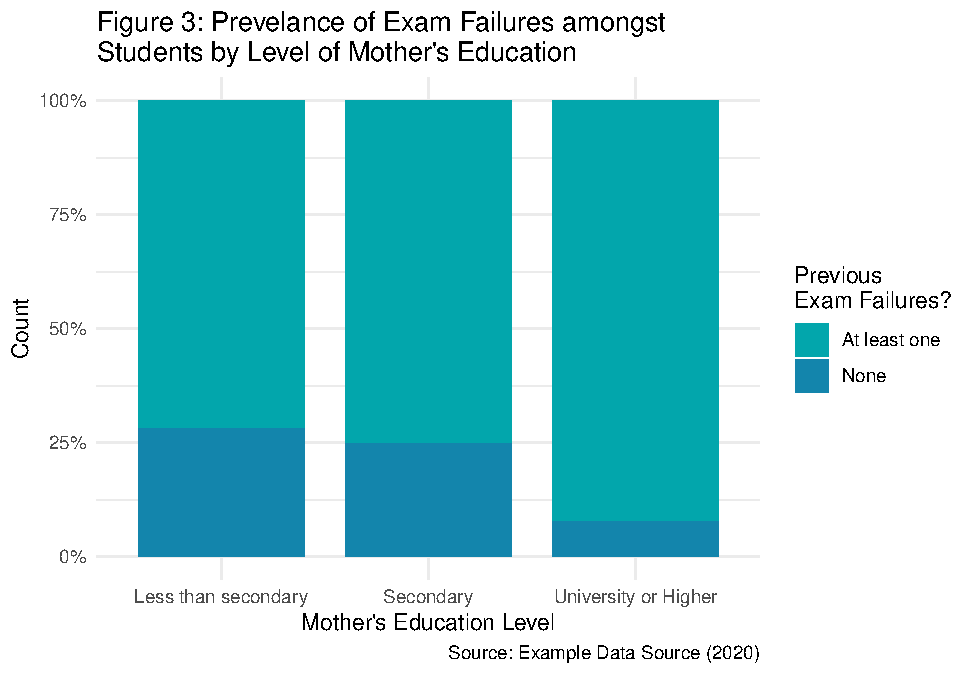
\includegraphics{bookdown-demo_files/figure-latex/unnamed-chunk-9-1.pdf}
\caption{\label{fig:unnamed-chunk-9}The colours set on this plot are far too similair}
\end{figure}

Previous advice already presented on the use of colour in graphs and maps (using it to highlight, use it sparingly etc.) are still relevant and contribute to ensuring accessibility. The advice presented here tends to focus on the choice of colours themselves.

\begin{itemize}
\item
  Ensure the colours are accessible.

  \begin{itemize}
  \item
    Colour blindness affects an individual's ability to distinguish between certain colours. It affects men more commonly than women.
  \item
    Most commonly, it affects the ability to distinguish reds and greens. Avoid using these colours together. Less commonly, but to be considered, is blue-yellow colour blindness. The two graphs below demonstrate how a colour-blind person may see a graph using red and green. The colours are much harder to distinguish.
  \item
    Red-green colour palettes may also not be clear when printed in greyscale.
  \item
    Blue palettes are a safe default starting point as they are colour blind safe and are visible in grayscale, as shown in the picture below.
  \end{itemize}
\end{itemize}

\begin{figure}
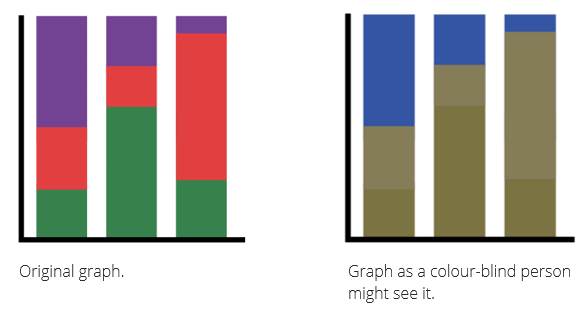
\includegraphics[width=1\linewidth]{img/colour_blind_graphs} \caption{A demonstration of how a colour-blind person would see a colourful graph}\label{fig:unnamed-chunk-10}
\end{figure}

\begin{figure}
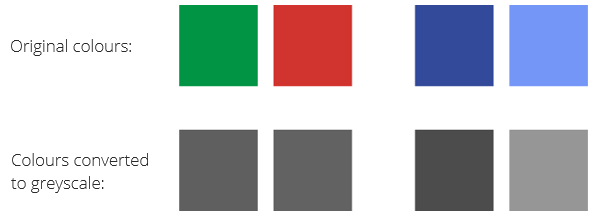
\includegraphics[width=1\linewidth]{img/colour_blind_2} \caption{Side by side comparison of colours converted to greyscale}\label{fig:unnamed-chunk-11}
\end{figure}

\begin{itemize}
\item
  Choose colours carefully.

  \begin{itemize}
  \tightlist
  \item
    Consider cultural context. Colours often have some inherent culturally defined associations. For instance, using colours people associate with familiar concepts can improve the quality and speed of information processing, such as using blue for water on a map.
  \end{itemize}
\end{itemize}

\begin{figure}
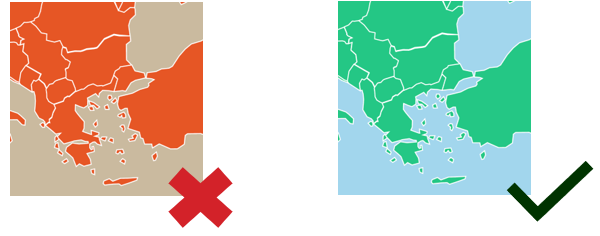
\includegraphics[width=1\linewidth]{img/cultural_context} \caption{Using colours logically}\label{fig:unnamed-chunk-12}
\end{figure}

\begin{itemize}
\item
  Understand the digital colour palette

  \begin{itemize}
  \tightlist
  \item
    Colours are represented using several common schemes. The most useful of these considers hue, saturation, and luminance. This scheme allows us to intuitively define unique colours.
  \end{itemize}
\item
  \textbf{Hue} -- Hues are colours. They do not have a natural order and therefore users cannot assign a logical order to them. Small changes in hue are easy to detect although colour blindness can affect how well people can detect these differences.
\end{itemize}

\begin{figure}

\includegraphics[width=1\linewidth]{img/visegs/eghue} \caption{Hue}\label{fig:unnamed-chunk-13}
\end{figure}

\begin{itemize}
\tightlist
\item
  \textbf{Saturation} -- This is the intensity of a colour, ranging from grey/white (no saturation) to rich, vibrant, almost glowing colour. Saturation is perceived on a continuous scale, although it is difficult to detect small changes. High saturation can also cause issues for those with certain visual/light sensitivity problems.
\end{itemize}

\begin{figure}

\includegraphics[width=1\linewidth]{img/visegs/egsat} \caption{Saturation}\label{fig:unnamed-chunk-14}
\end{figure}

\begin{itemize}
\tightlist
\item
  \textbf{Luminance} -- the brightness of colour. Also perceived as continuous ordered scale from dark to light. This natural order can help us optimize colour schemes for maximum distinction and differentiation.

  \begin{itemize}
  \tightlist
  \item
    Changes are easier to detect
  \item
    It is easier to distinguish between bars even if luminance is the only difference.
  \item
    Changes in luminance need to be larger if creating a line graph as the white space between the lines makes it harder to quickly compare.
  \end{itemize}
\end{itemize}

\begin{figure}

\includegraphics[width=1\linewidth]{img/visegs/eglum} \caption{Luminance}\label{fig:unnamed-chunk-15}
\end{figure}

\begin{itemize}
\tightlist
\item
  Never use an image as a background. This looks messy and cluttered and can make it difficult to read the graph.
\end{itemize}

\begin{figure}
\centering
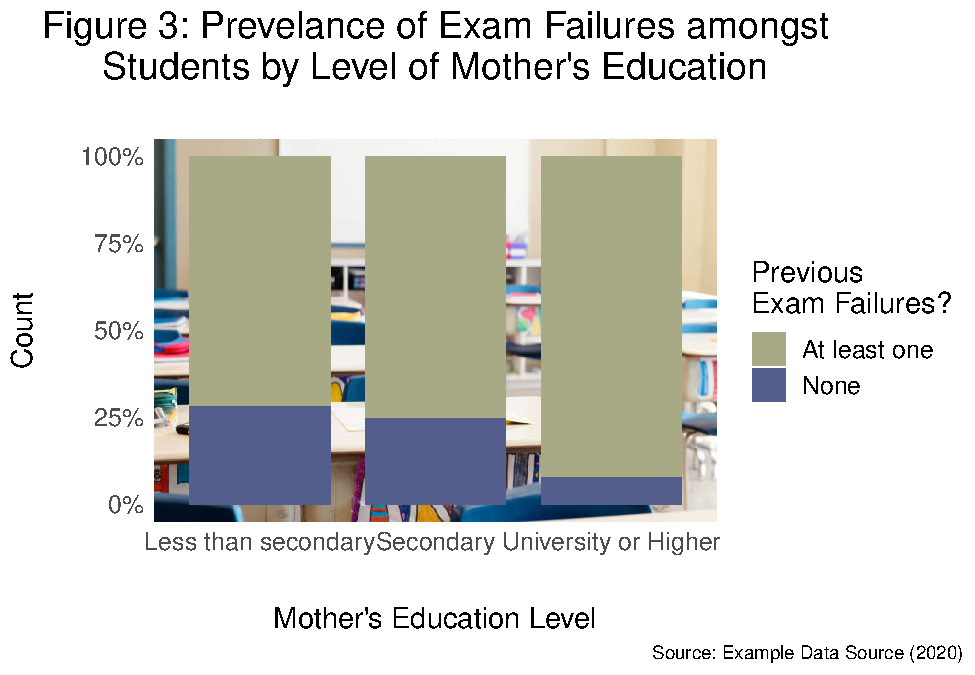
\includegraphics{bookdown-demo_files/figure-latex/unnamed-chunk-16-1.pdf}
\caption{\label{fig:unnamed-chunk-16}Using a background image in a plot}
\end{figure}

\begin{itemize}
\item
  Know how to use colour effectively

  \begin{itemize}
  \tightlist
  \item
    Alternate colours -- consider alternating dark and light for categorical data to improve clarity and distinction.
  \item
    Use borders -- adding thin borders to the edges of bars can enhance clarity/separation.
  \end{itemize}
\end{itemize}

\begin{figure}
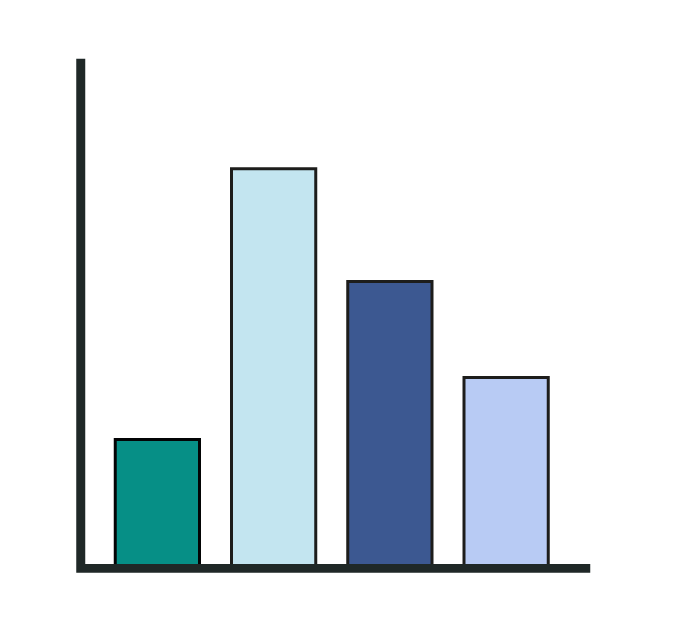
\includegraphics[width=1\linewidth]{img/visegs/egcolsgoodpractice} \caption{Use of alternating colours and borders}\label{fig:unnamed-chunk-17}
\end{figure}

\begin{itemize}
\tightlist
\item
  Avoid overuse of saturated colours.

  \begin{itemize}
  \tightlist
  \item
    Mid to low saturations are preferred
  \item
    Only use bold saturated colour to draw attention to a specific piece of information or hard to see, small elements.
  \item
    Bold, saturated colours can have visual side-effects. They may appear to glow for many users, can generate after-images and can affect how other colours appear.
  \end{itemize}
\end{itemize}

\begin{Shaded}
\begin{Highlighting}[]
\KeywordTok{ggplot}\NormalTok{(MathsGrades, }\KeywordTok{aes}\NormalTok{(}\DataTypeTok{x =}\NormalTok{ MotherEduc, }\DataTypeTok{fill =}\NormalTok{ Ever_fail))}\OperatorTok{+}
\StringTok{  }\KeywordTok{geom_bar}\NormalTok{(}\DataTypeTok{position =} \StringTok{"fill"}\NormalTok{, }\DataTypeTok{width =} \FloatTok{0.8}\NormalTok{)}\OperatorTok{+}
\StringTok{  }\KeywordTok{scale_fill_manual}\NormalTok{(}\DataTypeTok{values =} \KeywordTok{c}\NormalTok{(}\StringTok{"#03F8FF"}\NormalTok{, }\StringTok{"#FF3360"}\NormalTok{))}\OperatorTok{+}
\StringTok{  }\KeywordTok{scale_y_continuous}\NormalTok{(}\DataTypeTok{labels =}\NormalTok{ percent)}\OperatorTok{+}
\StringTok{  }\KeywordTok{labs}\NormalTok{(}\DataTypeTok{x =} \StringTok{"Mother's Education Level"}\NormalTok{,}
       \DataTypeTok{y =} \StringTok{"Count"}\NormalTok{,}
       \DataTypeTok{title =} \StringTok{"Figure 3: Prevelance of Exam Failures amongst}\CharTok{\textbackslash{}n}\StringTok{Students by Level of Mother's Education"}\NormalTok{,}
       \DataTypeTok{fill =} \StringTok{"Previous }\CharTok{\textbackslash{}n}\StringTok{Exam Failures?"}\NormalTok{,}
       \DataTypeTok{caption =} \StringTok{"Source: Example Data Source (2020)"}\NormalTok{)}\OperatorTok{+}
\StringTok{  }\KeywordTok{theme_minimal}\NormalTok{()}
\end{Highlighting}
\end{Shaded}

\begin{figure}
\centering
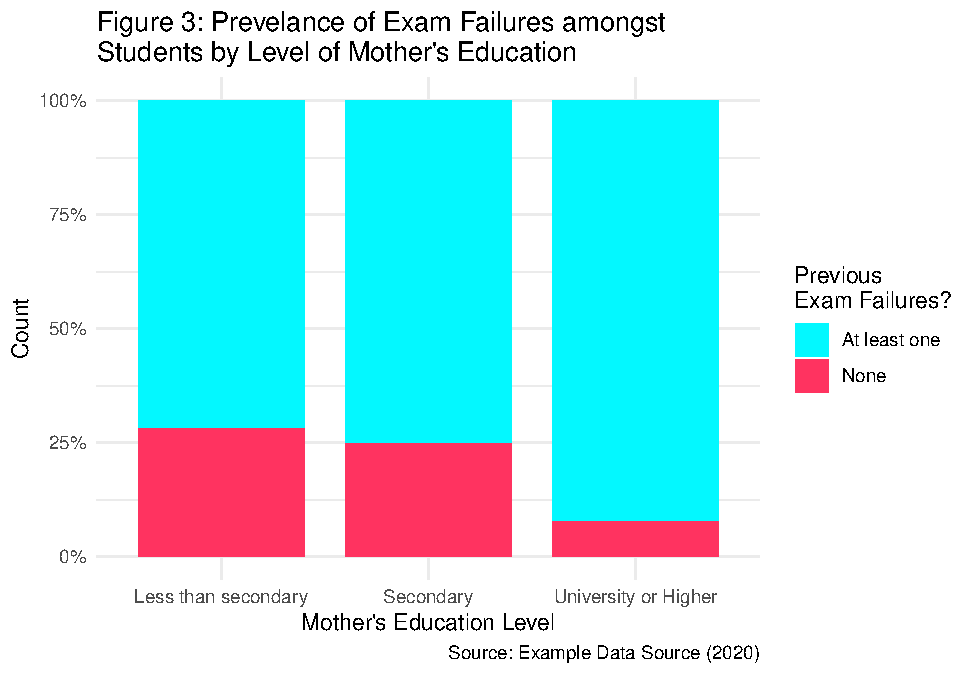
\includegraphics{bookdown-demo_files/figure-latex/unnamed-chunk-18-1.pdf}
\caption{\label{fig:unnamed-chunk-18}Over Saturated Colours on a graph}
\end{figure}

\begin{Shaded}
\begin{Highlighting}[]
\KeywordTok{ggplot}\NormalTok{(MathsGrades, }\KeywordTok{aes}\NormalTok{(}\DataTypeTok{x =}\NormalTok{ MotherEduc, }\DataTypeTok{fill =}\NormalTok{ Ever_fail))}\OperatorTok{+}
\StringTok{  }\KeywordTok{geom_bar}\NormalTok{(}\DataTypeTok{position =} \StringTok{"fill"}\NormalTok{, }\DataTypeTok{width =} \FloatTok{0.8}\NormalTok{, }\DataTypeTok{colour =} \StringTok{"black"}\NormalTok{)}\OperatorTok{+}
\StringTok{  }\KeywordTok{scale_fill_manual}\NormalTok{(}\DataTypeTok{values =} \KeywordTok{c}\NormalTok{(}\StringTok{"#60BDC0"}\NormalTok{, }\StringTok{"#C07384"}\NormalTok{))}\OperatorTok{+}
\StringTok{  }\KeywordTok{scale_y_continuous}\NormalTok{(}\DataTypeTok{labels =}\NormalTok{ percent)}\OperatorTok{+}
\StringTok{  }\KeywordTok{labs}\NormalTok{(}\DataTypeTok{x =} \StringTok{"Mother's Education Level"}\NormalTok{,}
       \DataTypeTok{y =} \StringTok{"Count"}\NormalTok{,}
       \DataTypeTok{title =} \StringTok{"Figure 3: Prevelance of Exam Failures amongst}\CharTok{\textbackslash{}n}\StringTok{Students by Level of Mother's Education"}\NormalTok{,}
       \DataTypeTok{fill =} \StringTok{"Previous }\CharTok{\textbackslash{}n}\StringTok{Exam Failures?"}\NormalTok{,}
       \DataTypeTok{caption =} \StringTok{"Source: Example Data Source (2020)"}\NormalTok{)}\OperatorTok{+}
\StringTok{  }\KeywordTok{theme_minimal}\NormalTok{()}
\end{Highlighting}
\end{Shaded}

\begin{figure}
\centering
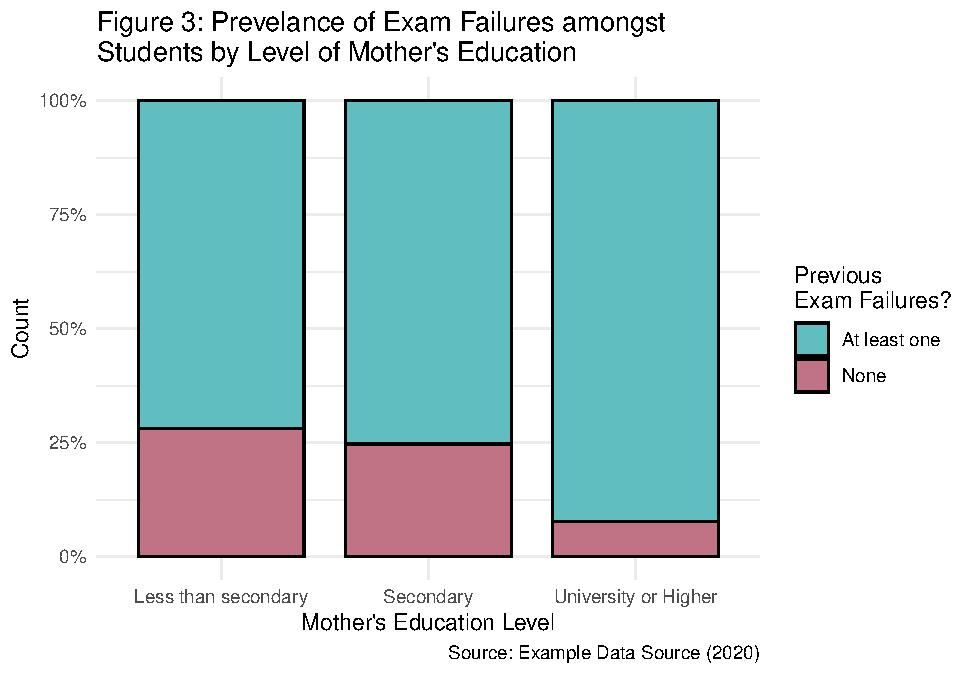
\includegraphics{bookdown-demo_files/figure-latex/unnamed-chunk-19-1.pdf}
\caption{\label{fig:unnamed-chunk-19}Low saturation makes the graph more pleasant to look at}
\end{figure}

\begin{itemize}
\item
  Use colour logically and consistently. If using sequences of colours, ensure that they progress in a logical manner that the user would expect, such as increasing luminance like in the map on page 50.

  \begin{itemize}
  \tightlist
  \item
    If creating multiple graphs, use the same colour to mean the same thing. Changing what they mean can confuse the user.
  \end{itemize}
\item
  Use a white background.

  \begin{itemize}
  \tightlist
  \item
    Most palettes are designed to appear on top of a white background. It provides a helpful reference for the colour scale being used.
  \end{itemize}
\end{itemize}

\hypertarget{using-colour-in-ggplot2}{%
\section{Using colour in ggplot2}\label{using-colour-in-ggplot2}}

ggplot2 comes with a wide array of capabilities to control the colour of various aspects of a graph. There are two main ways to add colour to a plot, either by allowing plotted objects (bar, points etc.) to vary according to a specified variable in your data or by simply setting something as a static colour.

To use a variable to define your colours, you include either \texttt{fill\ =\ variable} or \texttt{colour\ =\ variable} in the aesthetic mapping of your plot. \texttt{fill} refers to the space within objects/shapes such as the whitespace within a boxplot or a bar, while \texttt{colour} tends to refer to borders or points.

In the example below, we have assigned the \texttt{fill} of the column to vary according to the HHTYPE variable. Thereby turning the normal bar graph into a stacked bar graph.

\begin{Shaded}
\begin{Highlighting}[]
\KeywordTok{ggplot}\NormalTok{(BeanSurvey, }\KeywordTok{aes}\NormalTok{(}\DataTypeTok{x =}\NormalTok{ VILLAGE, }\DataTypeTok{y =}\NormalTok{ ADULTS, }\DataTypeTok{fill =}\NormalTok{ HHTYPE))}\OperatorTok{+}
\StringTok{  }\KeywordTok{geom_col}\NormalTok{()}
\end{Highlighting}
\end{Shaded}

\begin{figure}
\centering
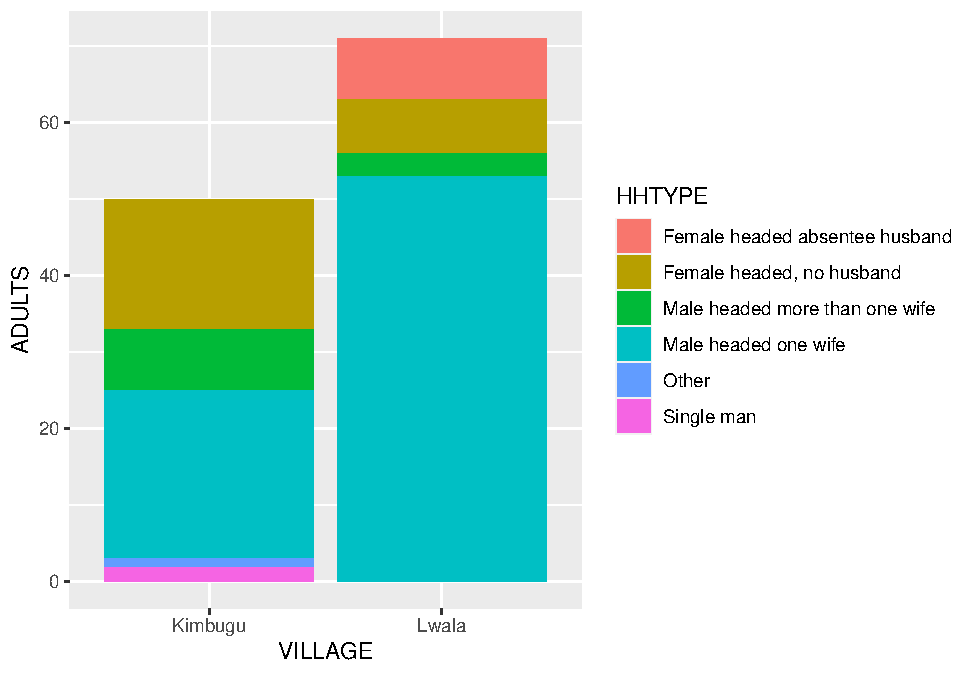
\includegraphics{bookdown-demo_files/figure-latex/unnamed-chunk-21-1.pdf}
\caption{\label{fig:unnamed-chunk-21}Using fill (barchart)}
\end{figure}

As we can see below the same idea does not really work if we tried the colour argument instead.

\begin{Shaded}
\begin{Highlighting}[]
\KeywordTok{ggplot}\NormalTok{(BeanSurvey, }\KeywordTok{aes}\NormalTok{(}\DataTypeTok{x =}\NormalTok{ VILLAGE, }\DataTypeTok{y =}\NormalTok{ ADULTS, }\DataTypeTok{colour =}\NormalTok{ HHTYPE))}\OperatorTok{+}
\StringTok{  }\KeywordTok{geom_col}\NormalTok{()}
\end{Highlighting}
\end{Shaded}

\begin{figure}
\centering
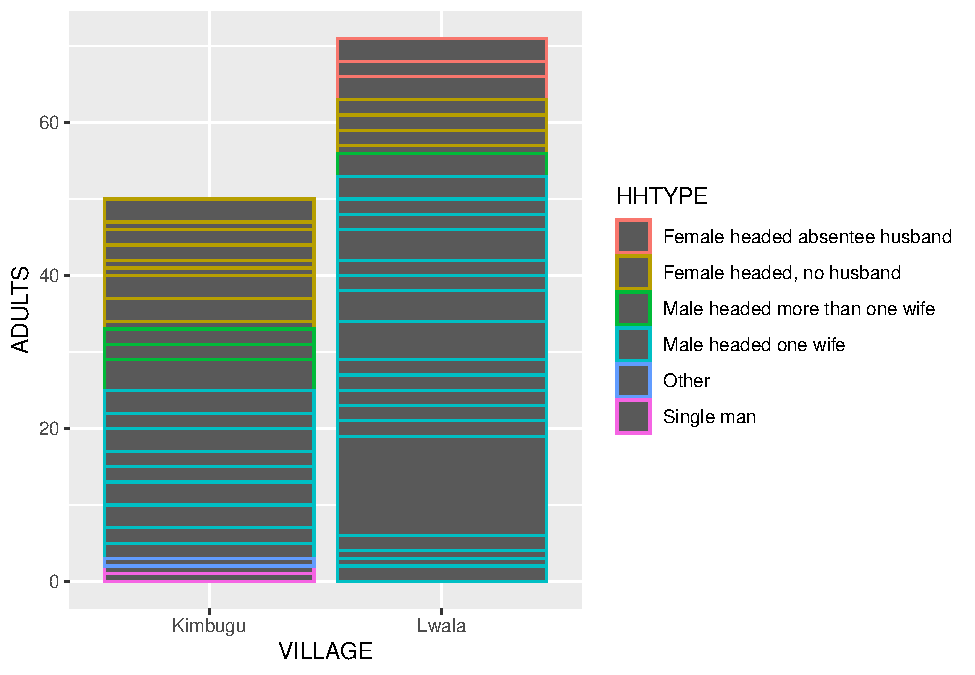
\includegraphics{bookdown-demo_files/figure-latex/unnamed-chunk-22-1.pdf}
\caption{\label{fig:unnamed-chunk-22}Using colour (barchart)}
\end{figure}

Colour is better suited to graphs such as a scatterplot. In this case the plot has been jittered to avoid overplotting.

\begin{Shaded}
\begin{Highlighting}[]
\KeywordTok{ggplot}\NormalTok{(MathsGrades, }\KeywordTok{aes}\NormalTok{(}\DataTypeTok{x =}\NormalTok{ Mock, }\DataTypeTok{y =}\NormalTok{ Final, }\DataTypeTok{colour =}\NormalTok{ Sex))}\OperatorTok{+}
\StringTok{  }\KeywordTok{geom_jitter}\NormalTok{()}
\end{Highlighting}
\end{Shaded}

\begin{figure}
\centering
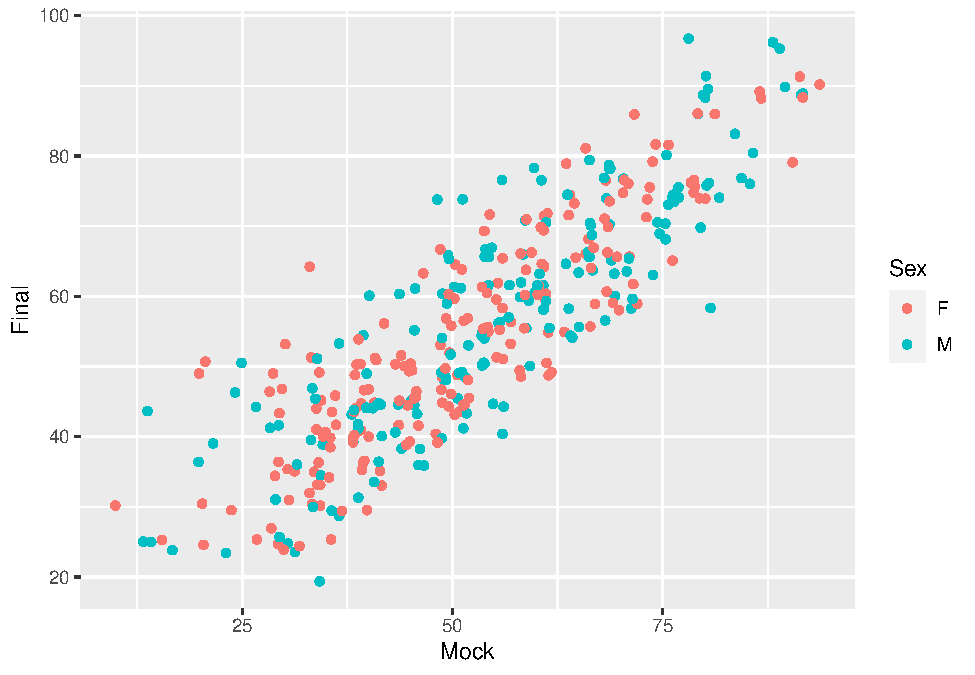
\includegraphics{bookdown-demo_files/figure-latex/unnamed-chunk-23-1.pdf}
\caption{\label{fig:unnamed-chunk-23}Using colour (scatter/jitterplot)}
\end{figure}

Again, this doesn't work when we try the reverse with fill.

\begin{Shaded}
\begin{Highlighting}[]
\KeywordTok{ggplot}\NormalTok{(MathsGrades, }\KeywordTok{aes}\NormalTok{(}\DataTypeTok{x =}\NormalTok{ Mock, }\DataTypeTok{y =}\NormalTok{ Final, }\DataTypeTok{fill =}\NormalTok{ Sex))}\OperatorTok{+}
\StringTok{  }\KeywordTok{geom_jitter}\NormalTok{()}
\end{Highlighting}
\end{Shaded}

\begin{figure}
\centering
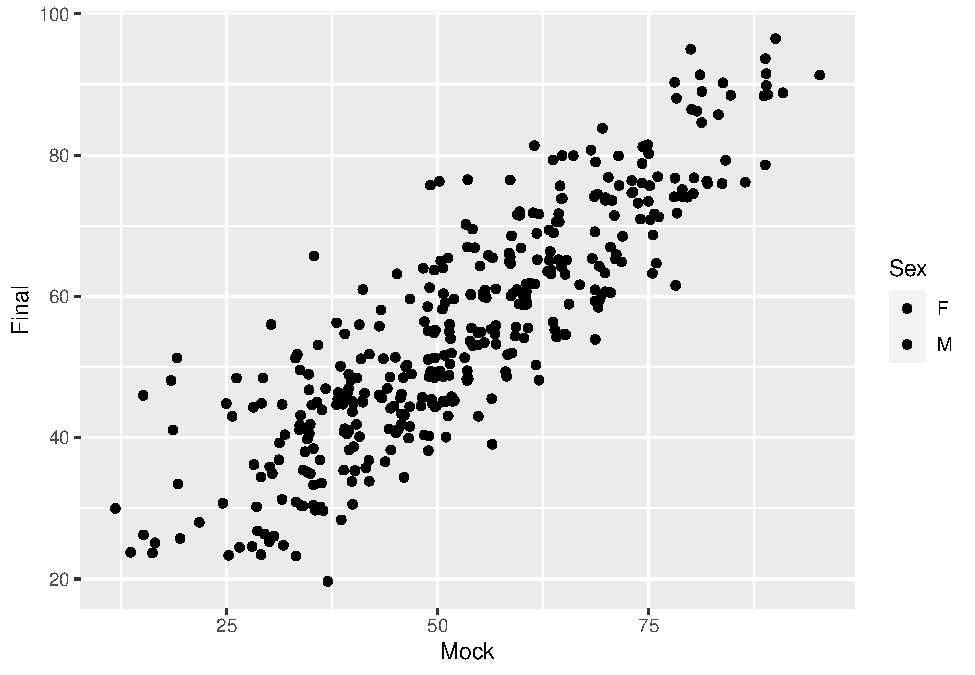
\includegraphics{bookdown-demo_files/figure-latex/unnamed-chunk-24-1.pdf}
\caption{\label{fig:unnamed-chunk-24}Using fill (scatter/jitterplot)}
\end{figure}

If we don't wish to allow colour to vary according to a variable in our data but rather set all objects to the same colour (other than the default grey/black), then we set the colour inside of the specific geom instead and not within a call to \texttt{aes()}. We can assign the colour using a hex code e.g.~\texttt{fill\ =\ "\#CD0000"} for a deep shade of red or by using the name of a pre-defined ggplot2 colour such as \texttt{colour\ =\ "dodgerblue4"}

\begin{Shaded}
\begin{Highlighting}[]
\KeywordTok{ggplot}\NormalTok{(BeanSurvey, }\KeywordTok{aes}\NormalTok{(}\DataTypeTok{x =}\NormalTok{ VILLAGE, }\DataTypeTok{y =}\NormalTok{ ADULTS))}\OperatorTok{+}
\StringTok{  }\KeywordTok{geom_col}\NormalTok{(}\DataTypeTok{fill =} \StringTok{"#CD0000"}\NormalTok{)}
\end{Highlighting}
\end{Shaded}

\begin{figure}
\centering
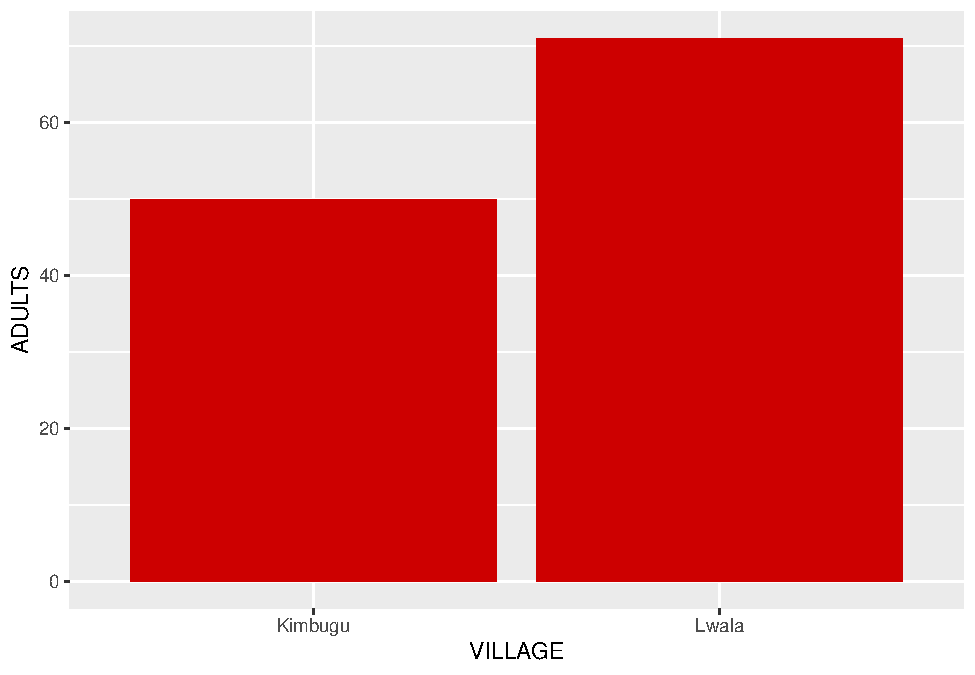
\includegraphics{bookdown-demo_files/figure-latex/unnamed-chunk-25-1.pdf}
\caption{\label{fig:unnamed-chunk-25}Setting fill with hex code}
\end{figure}

\begin{Shaded}
\begin{Highlighting}[]
\KeywordTok{ggplot}\NormalTok{(MathsGrades, }\KeywordTok{aes}\NormalTok{(}\DataTypeTok{x =}\NormalTok{ Mock, }\DataTypeTok{y =}\NormalTok{ Final))}\OperatorTok{+}
\StringTok{  }\KeywordTok{geom_jitter}\NormalTok{(}\DataTypeTok{colour =} \StringTok{"dodgerblue4"}\NormalTok{)}
\end{Highlighting}
\end{Shaded}

\begin{figure}
\centering
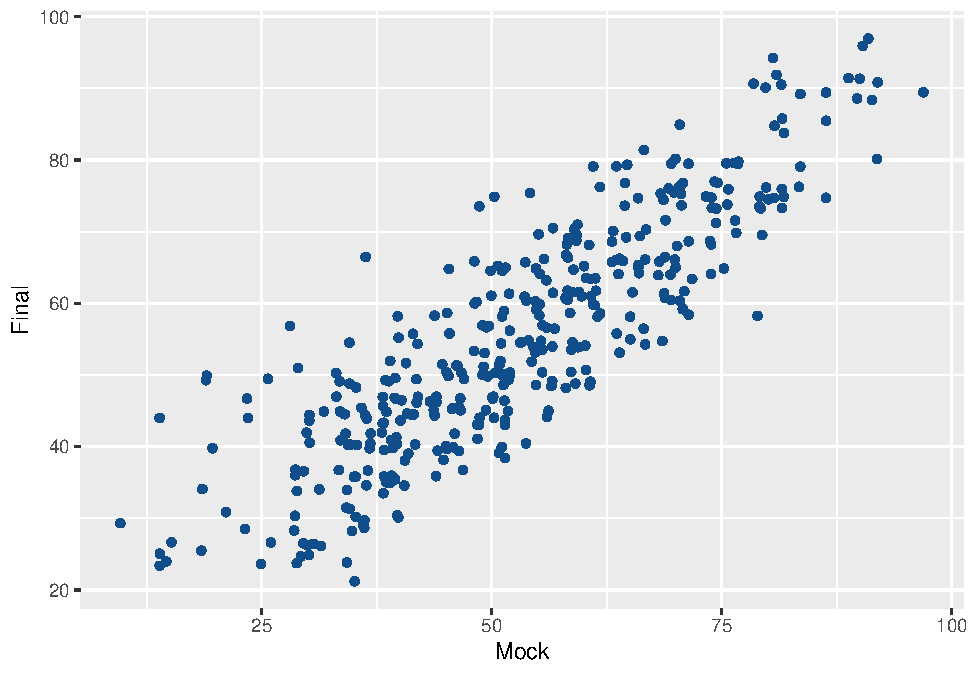
\includegraphics{bookdown-demo_files/figure-latex/unnamed-chunk-26-1.pdf}
\caption{\label{fig:unnamed-chunk-26}Setting colour with named colour}
\end{figure}

\hypertarget{changing-the-colourfill-scale}{%
\subsection{Changing the colour/fill scale}\label{changing-the-colourfill-scale}}

\hypertarget{setting-colours-manually}{%
\subsection{Setting colours manually}\label{setting-colours-manually}}

  \bibliography{book.bib,packages.bib}

\end{document}
